% =====================================================================
%  Расчётно-пояснительная записка к ВКР бакалавра
%  Тема: Разработка программно-аппаратного комплекса поддержки
%        мобильного приложения визуализации результатов работы
%        модификаций эволюционного алгоритма оптимизации
%  Автор: А.В. Волохов, ИУ9-82Б, МГТУ им. Н.Э. Баумана
%  Руководитель: Д.П. Посевин
%
%  Преамбула приведена в соответствие с разделом 10 Положения о ВКР:
%   - шрифт Times New Roman 14 pt (пакет tempora);
%   - полуторный межстрочный интервал;
%   - поля: левое 30 мм, правое 15 мм, верхнее 20 мм, нижнее 20 мм;
%   - абзацный отступ 1,25 см, выравнивание по ширине;
%   - номер страницы внизу по центру, верхний колонтитул пустой;
%   - рисунок: подпись снизу, «Рисунок N — Название»;
%   - таблица: подпись сверху, «Таблица N — Название»;
%   - формулы: сквозная нумерация, номер справа в круглых скобках.
%
%  Сборка: pdflatex -> biber -> pdflatex -> pdflatex
% =====================================================================

\documentclass[14pt, a4paper]{extarticle}

%%% Кодировки и язык %%%
\usepackage{cmap}
\usepackage[T2A]{fontenc}
\usepackage[utf8]{inputenc}
\usepackage[english, main=russian]{babel}

%%% Шрифт Times New Roman %%%
\usepackage{tempora}

%%% Поля страницы (Положение, п. 10.2) %%%
\usepackage{geometry}
\geometry{a4paper,
  left=30mm, right=15mm, top=20mm, bottom=20mm,
  headsep=10pt, footskip=12mm}

%%% Полуторный межстрочный интервал %%%
\usepackage{setspace}
\onehalfspacing

%%% Абзацный отступ 1,25 см и отступ у первого абзаца %%%
\usepackage{indentfirst}
\setlength{\parindent}{1.25cm}

%%% Математика %%%
\usepackage{amsmath, amssymb, amsfonts, mathtools}

%%% Таблицы %%%
\usepackage{array}
\usepackage{longtable}
\usepackage{multirow}
\usepackage{makecell}
\usepackage{tabularx}
\usepackage{booktabs}

%%% Рисунки %%%
\usepackage{graphicx}
\graphicspath{{figures/}}
\usepackage{float}

%%% Списки %%%
\usepackage{enumitem}
\setlist{nosep}
\renewcommand{\labelitemi}{---}

%%% Кавычки-ёлочки %%%
\usepackage{csquotes}
\DeclareQuoteStyle{russian}
  {\guillemotleft}{\guillemotright}[0.025em]
  {\quotedblbase}{\textquotedblleft}
\ExecuteQuoteOptions{style=russian}
\newcommand{\enq}[1]{\enquote{#1}}

%%% Десятичная запятая в формулах %%%
\usepackage{icomma}

%%% Подписи рисунков и таблиц (Положение, пп. 10.5, 10.6) %%%
\usepackage{caption}
\DeclareCaptionLabelSeparator{emdash}{~--~}
\captionsetup[figure]{labelsep=emdash, position=bottom, name=Рисунок,
  justification=centering, singlelinecheck=false}
\captionsetup[table]{labelsep=emdash, position=top, name=Таблица,
  justification=raggedright, singlelinecheck=false}

%%% Листинги кода (для приложений) — на пакете listings %%%
\usepackage{listings}
\usepackage{xcolor}
\definecolor{lstcomment}{rgb}{0.0,0.5,0.0}
\definecolor{lstkeyword}{rgb}{0.0,0.0,0.6}
\definecolor{lststring}{rgb}{0.58,0,0.82}
\renewcommand{\lstlistingname}{Листинг}
\lstset{
  basicstyle=\ttfamily\footnotesize,
  breaklines=true,
  breakatwhitespace=false,
  frame=single,
  numbers=left,
  numbersep=6pt,
  numberstyle=\footnotesize\color{gray},
  keywordstyle=\color{lstkeyword}\bfseries,
  commentstyle=\color{lstcomment},
  stringstyle=\color{lststring},
  showstringspaces=false,
  extendedchars=true,
  inputencoding=utf8,
  captionpos=t,
  xleftmargin=18pt,
  tabsize=4,
}

%%% Определение языка Dart для listings %%%
\lstdefinelanguage{Dart}{
  keywords={abstract, async, await, class, const, extends, final, for, if,
    import, in, new, return, super, switch, case, this, var, void, while,
    yield, get, set, late, required, factory, with, try, catch, rethrow,
    bool, int, double, String, true, false, null, Future, Stream, Map, List},
  keywordstyle=\color{lstkeyword}\bfseries,
  comment=[l]{//},
  morecomment=[s]{/*}{*/},
  commentstyle=\color{lstcomment},
  string=[b]',
  morestring=[b]",
  stringstyle=\color{lststring},
  sensitive=true,
}

%%% Колонтитулы: номер страницы внизу по центру, верх пустой (п. 10.3) %%%
\usepackage{fancyhdr}
\pagestyle{fancy}
\fancyhf{}
\renewcommand{\headrulewidth}{0pt}
\renewcommand{\footrulewidth}{0pt}
\fancyfoot[C]{\thepage}
\fancypagestyle{plain}{%
  \fancyhf{}\fancyfoot[C]{\thepage}%
  \renewcommand{\headrulewidth}{0pt}}

%%% Заголовки разделов (Положение, п. 10.4):
%%%   «глава/раздел» не пишется, в конце заголовка точки нет,
%%%   допускается полужирный шрифт, без переносов.
\usepackage[explicit]{titlesec}
\titleformat{\section}
  {\normalfont\large\bfseries\raggedright}{\thesection\quad}{0pt}{#1}
\titleformat{\subsection}
  {\normalfont\normalsize\bfseries\raggedright}{\thesubsection\quad}{0pt}{#1}
\titleformat{\subsubsection}
  {\normalfont\normalsize\bfseries\raggedright}{\thesubsubsection\quad}{0pt}{#1}
\titlespacing*{\section}{0pt}{12pt}{8pt}
\titlespacing*{\subsection}{0pt}{10pt}{6pt}
\titlespacing*{\subsubsection}{0pt}{8pt}{6pt}

% Каждая основная часть — с новой страницы
\newcommand{\sectionbreak}{\clearpage}

% Нумеровать подсекции (3.5.1) и включать их в оглавление
\setcounter{secnumdepth}{3}
\setcounter{tocdepth}{3}

%%% Ненумеруемый структурный элемент (заголовок прописными, по центру,
%%% с новой страницы, заносится в оглавление) — п. 9.3
\newcommand{\structelem}[1]{%
  \clearpage
  \phantomsection
  \addcontentsline{toc}{section}{#1}%
  \begin{center}\large\bfseries #1\end{center}
  \vspace{8pt}}

%%% Ссылки %%%
\usepackage[hidelinks]{hyperref}
\usepackage{cleveref}
\crefname{figure}{рисунок}{рисунки}
\crefname{table}{таблица}{таблицы}
\crefname{equation}{формула}{формулы}
\crefformat{equation}{(#2#1#3)}

%%% Библиография: biblatex + ГОСТ (Положение, п. 9.3 — ГОСТ 7.32) %%%
\usepackage[
  backend=biber,
  bibstyle=gost-numeric,
  citestyle=numeric-comp,
  sorting=none,
  language=russian
]{biblatex}
\AtEveryBibitem{\clearfield{isbn}\clearfield{issn}}
\addbibresource{biblio.bib}

%%% Перенос слов и борьба с висячими строками %%%
\sloppy
\clubpenalty=10000
\widowpenalty=10000

% =====================================================================
\begin{document}


\begin{titlepage}
\thispagestyle{empty}
\newpage

\vspace*{-30pt}
\hspace{-45pt}
\begin{minipage}{0.17\textwidth}
\hspace*{-20pt}\centering

\includegraphics[width=1.3\textwidth]{emblem.png}
\end{minipage}
\begin{minipage}{0.82\textwidth}\small \textbf{
\vspace*{-0.7ex}
\hspace*{-10pt}\centerline{Министерство науки и высшего образования Российской Федерации}
\vspace*{-0.7ex}
\centerline{Федеральное государственное автономное образовательное учреждение}
\vspace*{-0.7ex}
\centerline{высшего образования}
\vspace*{-0.7ex}
\centerline{<<Московский государственный технический университет}
\vspace*{-0.7ex}
\centerline{имени Н.Э. Баумана}
\vspace*{-0.7ex}
\centerline{(национальный исследовательский университет)>>}
\vspace*{-0.7ex}
\centerline{(МГТУ им. Н.Э. Баумана)}}
\end{minipage}

\vspace{-2pt}
\hspace{-34.5pt}\rule{\textwidth}{2.5pt}

\vspace*{-20.3pt}
\hspace{-34.5pt}\rule{\textwidth}{0.4pt}

\vspace{0.5ex}
\noindent \small ФАКУЛЬТЕТ\hspace{80pt} <<Информатика и системы управления>>

\vspace*{-16pt}
\hspace{35pt}\rule{0.855\textwidth}{0.4pt}

\vspace{0.5ex}
\noindent \small КАФЕДРА\hspace{50pt} <<Теоретическая информатика и компьютерные технологии>>

\vspace*{-16pt}
\hspace{25pt}\rule{0.875\textwidth}{0.4pt}

\vspace{3em}

\begin{center}
\Large \bfseries
РАСЧЕТНО-ПОЯСНИТЕЛЬНАЯ ЗАПИСКА\\
\textit{К ПРЕДДИПЛОМНОЙ ПРАКТИКЕ\\НА ТЕМУ:}
\end{center}

\vspace*{-2.5ex}
\begin{center}
\newcommand{\TitleLine}[1]{%
  \underline{\makebox[0.9\textwidth][c]{\Large\textit{\textbf{#1}}}}%
  \par\vspace{0.9ex}%
}
\TitleLine{Разработка программно-аппаратного комплекса}
\TitleLine{поддержки мобильного приложения визуализации}
\TitleLine{результатов работы модификаций эволюционного}
\TitleLine{алгоритма оптимизации}
\TitleLine{}
\end{center}

\vspace{\fill}

\newlength{\ML}
\settowidth{\ML}{«\underline{\hspace{0.7cm}}» \underline{\hspace{2cm}}}

\newcommand{\ulfield}[2]{%
  \underline{\makebox[#1][c]{\raisebox{0pt}[1.6ex][0pt]{#2}}}%
}

\noindent Студент\quad \ulfield{1.5cm}{ИУ9-82Б} \hfill
\ulfield{4cm}{}\quad
\ulfield{4cm}{А.В.~Волохов}

\vspace{-2.1ex}
\noindent\hspace{9ex}\scriptsize{(Группа)}\normalsize\hspace{170pt}\hspace{2ex}%
\scriptsize{(Подпись, дата)}\normalsize\hspace{30pt}\hspace{6ex}%
\scriptsize{(И.О. Фамилия)}\normalsize

\bigskip

\noindent Руководитель практики \hfill
\ulfield{4cm}{}\quad
\ulfield{4cm}{Д.П.~Посевин}

\vspace{-2ex}
\noindent\hspace{13.5ex}\normalsize\hspace{170pt}\hspace{2ex}%
\scriptsize{(Подпись, дата)}\normalsize\hspace{30pt}\hspace{6ex}%
\scriptsize{(И.О. Фамилия)}\normalsize
\vfill

\begin{center}
\textsl{\the\year{} г.}
\end{center}
\end{titlepage}

% Содержание начинается со страницы 3. При ином числе бланков изменить число ниже.
\setcounter{page}{2}

% =====================================================================
%  СОДЕРЖАНИЕ
% =====================================================================
\clearpage
\phantomsection
\renewcommand{\contentsname}{\centerline{\large\bfseries СОДЕРЖАНИЕ}}
\tableofcontents

% =====================================================================
%  СПИСОК ОБОЗНАЧЕНИЙ И СОКРАЩЕНИЙ
% =====================================================================
\structelem{СПИСОК ОБОЗНАЧЕНИЙ И СОКРАЩЕНИЙ}

В настоящей РПЗ применяют следующие сокращения и обозначения.

\begin{description}[leftmargin=!, labelwidth=2.6cm, font=\normalfont, itemsep=2pt]
  \item[BBO] --- алгоритм биогеографической оптимизации (Biogeography-Based Optimization)
  \item[GIF] --- формат обмена графическими данными (Graphics Interchange Format)
  \item[HSI] --- индекс пригодности среды обитания (Habitat Suitability Index)
  \item[HTTP] --- протокол передачи гипертекста (Hypertext Transfer Protocol)
  \item[JSON] --- текстовый формат обмена данными (JavaScript Object Notation)
  \item[PSO] --- метод роя частиц (Particle Swarm Optimization)
  \item[TCP] --- протокол управления передачей (Transmission Control Protocol)
  \item[WebSocket] --- протокол полнодуплексной связи поверх TCP
\end{description}

\structelem{ОПИСАНИЕ БАЗЫ ПРАКТИКИ}

Местом прохождения практики является Отдел информационных технологий и
поддержки (ОИТП) МГТУ им.~Н.Э.~Баумана --- структурное подразделение,
обеспечивающее работу информационно-технологической инфраструктуры
всего университетского комплекса. В зону ответственности отдела входит
широкий круг задач: техническая поддержка пользователей,
администрирование корпоративной сети и серверного оборудования, а
также поддержка и развитие информационных систем университета.

Деятельность ОИТП охватывает как повседневную эксплуатацию цифровых
сервисов --- систем аутентификации, учебных порталов, систем
документооборота, --- так и задачи по внедрению новых программных
решений в интересах образовательного и административного процессов.
Специалисты отдела обеспечивают бесперебойный доступ к инфраструктуре
для преподавателей, студентов и сотрудников университета.


% =====================================================================
%  ВВЕДЕНИЕ — ~1 страница, без подразделов, не нумеруется
% =====================================================================
\structelem{ВВЕДЕНИЕ}

Многие практические задачи сводятся к поиску глобального минимума целевой
функции. Часто у такой функции, помимо глобального минимума, есть множество
локальных. Классические градиентные методы здесь малоэффективны: они сходятся
к ближайшему локальному минимуму и не умеют из него выбираться. Поэтому для
функций с множеством локальных минимумов применяют метаэвристические алгоритмы,
которые работают сразу с целой популяцией решений~\cite{karpenko2021}. Один из
них --- алгоритм биогеографической оптимизации (Biogeography-Based
Optimization, далее --- BBO)~\cite{simon2020, karpenko2013bbo}.

Поведение метаэвристик трудно предсказать аналитически, поэтому об их работе
чаще судят по результатам запусков. Здесь многое даёт визуализация: по ней
видно, как убывает лучшее найденное значение, как популяция распределяется в
пространстве решений и не наступает ли преждевременная сходимость. Удобно, когда
такой инструмент доступен прямо на мобильном устройстве и не требует настройки
вычислительного окружения. Этим и обусловлена актуальность работы.

Объект исследования --- модификации алгоритма биогеографической оптимизации,
а также метод роя частиц, который привлекается для сравнения. Программа
рассчитана прежде всего на студентов, изучающих методы оптимизации, и на
исследователей, которым нужно быстро сравнить поведение разных метаэвристик на
тестовых задачах.

Цель работы --- разработка программно-аппаратного комплекса поддержки мобильного
приложения визуализации результатов работы модификаций эволюционного алгоритма
оптимизации. Для её достижения решается несколько связанных между собой задач.

Вычисления выполняет серверное ядро. Оно должно поддерживать целое семейство
методов: классический BBO, его варианты с синусоидальной и смешанной моделями
миграции, их модификации с адаптивной мутацией, перезапуском при стагнации и
локальным поиском, а также метод роя частиц. Запускать алгоритмы нужно как на
стандартных тестовых функциях, так и на функции, которую пользователь задаёт
собственным выражением.

Чтобы мобильное устройство могло ставить задачи серверу и получать от него
данные, нужен протокол обмена. Он должен поддерживать постановку задачи, передачу
прогресса по итерациям в реальном времени, выдачу итогового результата, отмену
задачи и работу очереди, когда клиентов несколько.

С пользователем взаимодействует мобильное приложение. Через него настраивают
эксперимент, отправляют задачу на сервер и следят за ходом вычислений и итогом.

Главное в приложении --- наглядно показать, как работает алгоритм. Для этого
строится график сходимости в реальном времени, пространство поиска отображается
контурной картой и трёхмерной поверхностью, а динамика популяции --- анимацией.

Смысл комплекса в том, чтобы сравнивать методы, поэтому история запусков
сохраняется. Сохранённые результаты можно сопоставлять --- на совмещённых
графиках и в таблице.

% =====================================================================
%  2. КОНСТРУКТОРСКАЯ ЧАСТЬ
% =====================================================================
\section{Конструкторская часть}\label{sec:design}

\subsection{Функциональные требования к программному комплексу}
\label{subsec:requirements}

Прежде чем переходить к проектированию, нужно определить, что комплекс должен
делать. Требования удобно разделить на функциональные, описывающие возможности
системы с точки зрения пользователя, и нефункциональные, задающие общие свойства
системы.

Основной сценарий работы --- постановка и проведение вычислительного эксперимента.
Пользователь должен иметь возможность выбрать метод оптимизации из доступного
семейства, задать целевую функцию и параметры задачи, после чего запустить
вычисление. В качестве целевой функции система должна принимать как одну из
встроенных тестовых функций, так и произвольное выражение, введённое
пользователем. Для задачи пользователь должен задавать размерность и границы
области поиска, а для выбранного метода --- его параметры, например размер
популяции, число поколений и вероятность мутации.

Во время вычисления система должна показывать ход поиска, не дожидаясь его
завершения. Пользователю нужно видеть номер текущего поколения, лучшее найденное
значение целевой функции и график сходимости, который обновляется по мере
поступления новых данных. Кроме того, должна быть возможность отменить запущенную
задачу и видеть положение задачи в очереди, если она ещё не начала выполняться.

После завершения эксперимента система должна представить его результат: лучшее
найденное решение и значение функции в нём, график сходимости за весь запуск,
а также числовые показатели качества. Для наглядного представления пространства
поиска результат должен сопровождаться визуализацией: контурной картой целевой
функции с нанесёнными на неё решениями, трёхмерной поверхностью функции с
возможностью её вращения и анимацией, показывающей, как менялась популяция от
поколения к поколению.

Способы визуализации накладывают на систему ряд требований. Прежде всего график 
сходимости должен обновляться инкрементально: новые точки добавляются к уже 
построенной кривой по мере поступления данных, а не строятся каждый раз заново. 
Это необходимо, чтобы пользователь видел ход поиска во время вычислений, и одновременно 
снижает нагрузку на устройство. Затем, поскольку экран смартфона невелик, представление данных
должно быть лаконичным: с читаемыми подписями осей и легендой, не перекрывающей
основной график. Наконец, построение контурной карты и трёхмерной поверхности
требует многократного вычисления целевой функции, поэтому карта и поверхность
должны рассчитываться один раз, а при наблюдении за поиском и вращении должны
обновляться только положения маркеров и точка обзора, но не сам рельеф.

Результаты экспериментов должны сохраняться, чтобы пользователь мог вернуться к
ним позже. Система должна хранить историю проведённых запусков и позволять
просматривать её, отбирать отдельные запуски и сравнивать несколько результатов
между собой --- на совмещённом графике сходимости, в виде таблицы показателей и
столбчатой диаграммы.

Нефункциональные требования определяются назначением системы и условиями её
использования. Поскольку основным устройством пользователя является смартфон,
приложение должно работать на мобильной платформе и оставаться отзывчивым:
интерфейс не должен подвисать во время вычислений и построения графиков. Сами
вычисления могут быть длительными и ресурсоёмкими, поэтому их следует выполнять
отдельно от устройства пользователя, на сервере. Сервер, в свою очередь, должен
поддерживать одновременную работу нескольких клиентов и упорядочивать поступающие
от них задачи.

\subsection{Архитектура программного комплекса}
\label{subsec:architecture}

Перечисленные возможности естественно распределяются между двумя разными по
назначению частями системы. Одна обращена к пользователю и должна работать на
смартфоне, другая выполняет ресурсоёмкие вычисления. Совмещать их в одном
приложении нецелесообразно: оптимизация на больших популяциях и высоких
размерностях нагружает процессор, а мобильное устройство ограничено по
вычислительной мощности и расходу батареи. Поэтому выбрана клиент-серверная
архитектура, в которой вычисления вынесены на сервер, а мобильное приложение
отвечает за управление и отображение результатов~\cite{olifer2016}. Общая
структура комплекса показана на рисунке~\ref{fig:architecture}.

\begin{figure}[H]
  \centering
  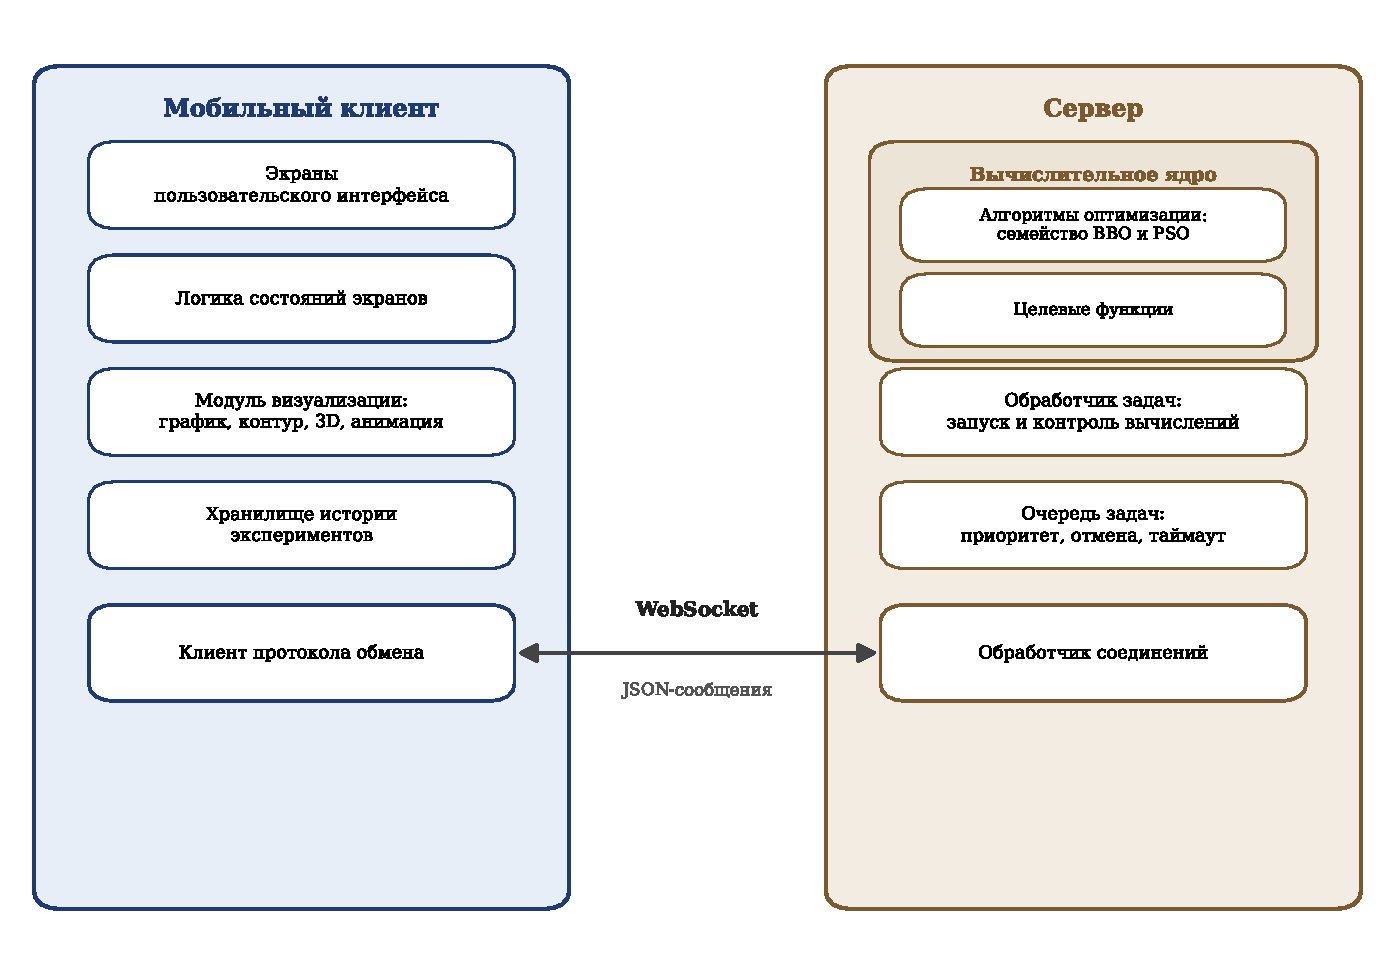
\includegraphics[width=0.92\linewidth]{architecture.pdf}
  \caption{Архитектура программного комплекса}
  \label{fig:architecture}
\end{figure}

Мобильный клиент --- это приложение, с которым непосредственно работает
пользователь. Оно состоит из нескольких слоёв. Экраны образуют пользовательский
интерфейс: настройку эксперимента, наблюдение за прогрессом, просмотр результата
и работу с историей. За экранами стоит слой логики состояний, который хранит
текущее состояние каждого экрана и реагирует на действия пользователя и на данные,
приходящие с сервера. Отдельный модуль отвечает за визуализацию --- построение
графика сходимости, контурной карты, трёхмерной поверхности и анимации. История
проведённых экспериментов хранится в локальной базе данных на самом устройстве,
что позволяет работать с прошлыми результатами и без подключения к серверу.
Наконец, клиент протокола обмена обеспечивает связь с сервером.

Сервер выполняет вычисления и не имеет собственного интерфейса. Все запросы
клиентов принимает обработчик соединений: он разбирает входящие сообщения и
направляет их дальше. Поскольку клиентов может быть несколько, а вычисления
длительны, поступающие задачи помещаются в очередь, которая упорядочивает их и
позволяет отменять ещё не выполненные. Выполнением занимается обработчик задач:
он берёт задачу из очереди, запускает соответствующий алгоритм и по ходу работы
отправляет клиенту данные о прогрессе. Сами алгоритмы оптимизации --- семейство
BBO и метод роя частиц --- вместе с целевыми функциями образуют вычислительное
ядро сервера. Какой именно алгоритм запускать и какую функцию вычислять,
обработчик задач определяет по сведениям из поступившего запроса.

Взаимодействие между клиентом и сервером построено поверх протокола WebSocket.
В отличие от обычного запроса и ответа по протоколу HTTP, WebSocket держит
постоянное двустороннее соединение, по которому сервер может в любой момент
присылать клиенту новые данные~\cite{fedulov2025, rfc6455}. Это и нужно для передачи
прогресса: пока идёт вычисление, сервер по тому же соединению отправляет клиенту
сведения о каждом поколении, и приложение обновляет график сходимости в реальном
времени. Сообщения передаются в текстовом формате JSON, общая структура которого
описана в следующем подразделе.

\subsection{Проектирование протокола обмена данными}
\label{subsec:protocol-design}

Клиент и сервер обмениваются сообщениями по постоянному соединению WebSocket.
Чтобы этот обмен был упорядоченным и расширяемым, нужен прикладной протокол ---
набор правил о том, какие сообщения бывают, как они устроены и в каком порядке
ими обмениваются. Все сообщения протокола передаются в текстовом формате
JSON~\cite{rfc8259}. Этот формат выбран потому, что он удобочитаем, поддерживается без дополнительных
библиотек в типовых веб-приложениях, и его разбор встроен в стандартные средства
как серверного, так и клиентского языка~\cite{shulman2021}.

Каждое сообщение имеет единую структуру и состоит из двух частей --- заголовка и
полезной нагрузки. Заголовок содержит служебные поля, общие для всех сообщений:
версию протокола, тип сообщения, его уникальный идентификатор, метку времени, а
также поля для связи сообщений между собой и для идентификации задачи. Полезная
нагрузка зависит от типа сообщения и содержит его данные: например, параметры
запускаемой задачи или сведения об очередном поколении. Такое разделение
позволяет обрабатывать служебную часть единообразно, не разбирая каждый тип
сообщения по-своему.

Все сообщения делятся на несколько групп по назначению. Служебные сообщения
обслуживают само соединение:
\begin{itemize}
  \item \texttt{hello} --- рукопожатие при подключении и обмен сведениями о
  возможностях сторон;
  \item \texttt{ping} и \texttt{pong} --- проверка того, что соединение живо;
  \item \texttt{error} --- сообщение об ошибке протокола, проверки данных или
  выполнения.
\end{itemize}

Сообщения управления задачами обеспечивают её постановку и сопровождение:
\begin{itemize}
  \item \texttt{job.submit} --- запрос на запуск задачи с указанием метода,
  целевой функции и параметров;
  \item \texttt{job.accepted} --- подтверждение приёма задачи и присвоение ей
  идентификатора;
  \item \texttt{cancel} --- запрос на отмену задачи;
  \item \texttt{job.status.get} и \texttt{job.status} --- запрос текущего
  состояния задачи и ответ на него.
\end{itemize}

Сообщения о ходе и итогах вычисления идут от сервера к клиенту:
\begin{itemize}
  \item \texttt{job.started} --- уведомление о начале выполнения задачи;
  \item \texttt{job.progress} --- данные об очередном поколении: его номер и
  лучшее найденное значение;
  \item \texttt{job.result} --- итоговый результат с лучшим решением и
  показателями качества;
  \item \texttt{job.finished} --- уведомление о завершении задачи с указанием
  итогового состояния.
\end{itemize}

Порядок, в котором сервер меняет состояние задачи и шлёт эти сообщения, образует
жизненный цикл задачи. Он показан на рисунке~\ref{fig:lifecycle}. Поступившая
задача сначала попадает в очередь. Когда обработчик задач берёт её в работу, она
переходит в состояние выполнения, и клиенту отправляется уведомление о начале.
Во время выполнения сервер периодически шлёт сообщения о прогрессе. Завершиться
задача может по-разному: успешно, с ошибкой, по отмене пользователем или по
превышению отведённого времени. Отменить задачу можно и пока она ещё стоит в
очереди.

\begin{figure}[H]
  \centering
  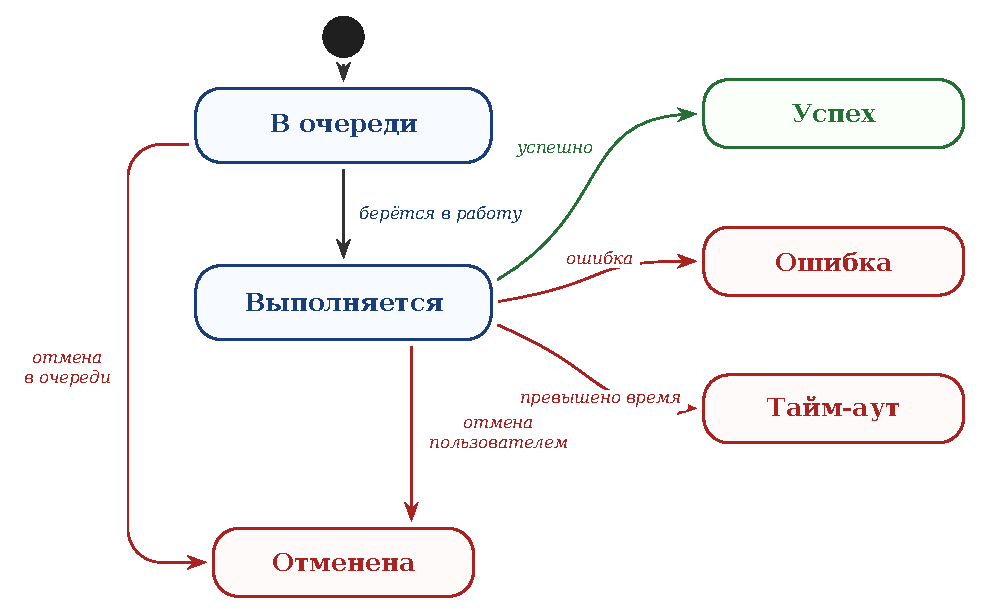
\includegraphics[width=0.92\linewidth]{job_lifecycle.pdf}
  \caption{Жизненный цикл задачи на сервере}
  \label{fig:lifecycle}
\end{figure}

В протоколе предусмотрены и средства для передачи больших объёмов данных. Если
сообщение превышает допустимый размер, его полезную нагрузку можно разбить на
части --- чанки --- и собрать на стороне клиента по общему идентификатору потока.
Аналогично заголовок предусматривает возможность сжатия полезной нагрузки. Эти
средства заложены в протокол на будущее: при текущих объёмах данных, которыми
обмениваются клиент и сервер, разбиение на части и сжатие не требуются, и
сообщения передаются целиком в несжатом виде.

\subsection{Модель хранения данных}
\label{subsec:data-model}

Одно из требований к системе --- сохранять историю проведённых экспериментов,
чтобы пользователь мог возвращаться к прошлым запускам и сравнивать их между
собой. Отсюда вытекает несколько задач, которые должно решать хранилище. Во-первых,
по каждому запуску нужно сохранять достаточно сведений, чтобы его можно было
однозначно опознать в списке и понять, что именно вычислялось: каким методом,
на какой задаче и с каким итогом. Во-вторых, нужно хранить сам результат запуска ---
не только итоговое число, но и данные, по которым строятся графики и визуализация,
иначе к завершённому эксперименту нельзя будет вернуться позже. В-третьих, записи
должны быть однородными, чтобы их можно было перебирать, отбирать по условию и
сопоставлять друг с другом.

Чтобы учесть эти требования, прежде всего нужно понять, какие данные и в каких
отношениях между собой следует хранить. Для этого построена концептуальная модель
данных в виде диаграммы \enq{сущность-связь}, показанная на
рисунке~\ref{fig:er-model}. Она описывает предметную область на уровне сущностей и
связей, без привязки к конкретному способу хранения.

\begin{figure}[H]
  \centering
  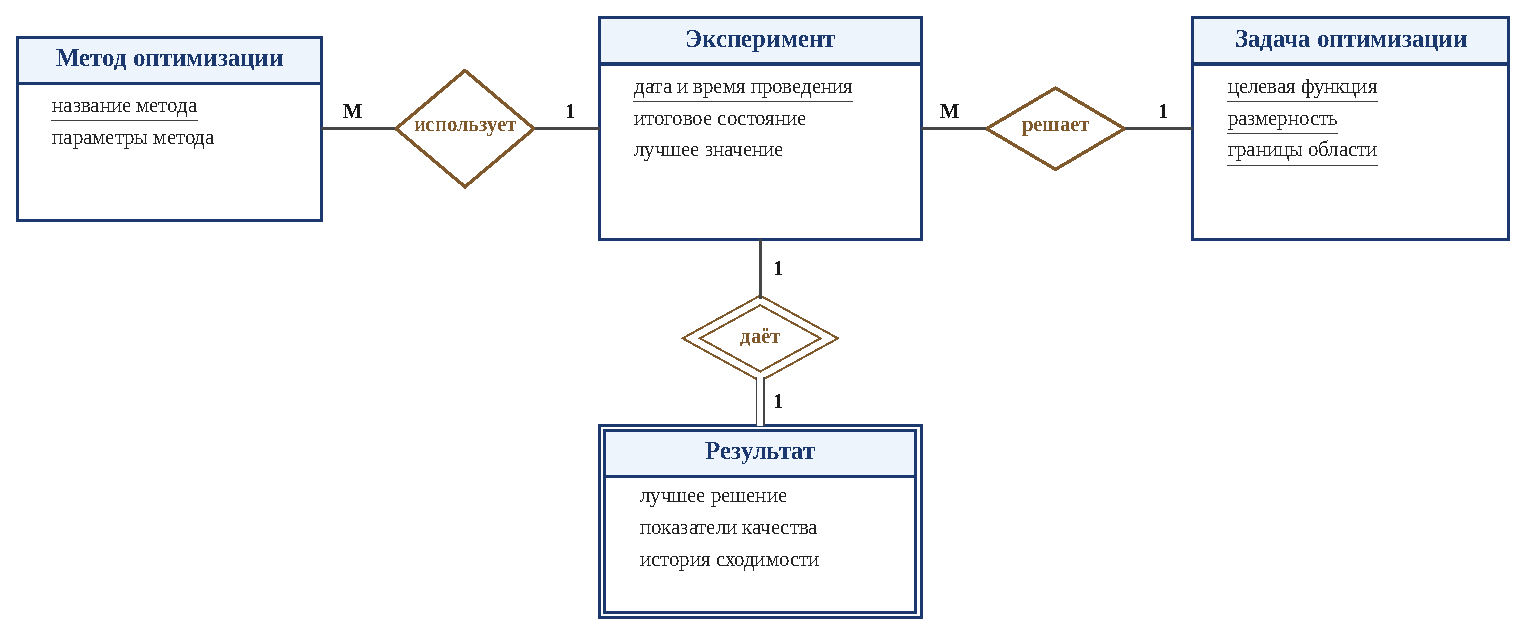
\includegraphics[width=0.95\linewidth]{er_model.pdf}
  \caption{Модель \enq{сущность-связь} истории экспериментов}
  \label{fig:er-model}
\end{figure}

Центральная сущность модели --- эксперимент. Он соответствует одному завершённому
запуску оптимизации и описывается идентификатором, датой проведения, итоговым
состоянием и лучшим найденным значением целевой функции. Идентификатор является
ключевым атрибутом: он однозначно определяет запись об эксперименте.

С экспериментом связаны три другие сущности. Метод оптимизации описывает, каким
алгоритмом проводился запуск, и хранит название метода и значения его параметров.
Один и тот же метод может использоваться во многих экспериментах, поэтому связь
\enq{использует} имеет тип <<многие к одному>>. Задача оптимизации описывает, что
именно решалось: целевую функцию, размерность и границы области поиска. Одна и та
же задача также может встречаться в разных экспериментах, поэтому связь
\enq{решает} тоже имеет тип <<многие к одному>>. Наконец, результат хранит итог
запуска: лучшее найденное решение, числовые показатели качества и историю
сходимости, по которой строится график. Каждому эксперименту соответствует ровно
один результат, поэтому связь \enq{даёт} имеет тип <<один к одному>>.

Такая модель отражает естественную структуру предметной области: эксперимент
объединяет вокруг себя сведения о применённом методе, решаемой задаче и полученном
результате. История экспериментов представляет собой набор однородных записей
такого вида, который пополняется после каждого завершённого запуска и хранится на
устройстве пользователя.

\subsection{Проектирование пользовательского интерфейса}
\label{subsec:ui-design}

Интерфейс приложения строится вокруг основного сценария работы: настроить
эксперимент, запустить его, понаблюдать за ходом вычислений и изучить результат.
Чтобы каждый шаг этого сценария был понятен и не перегружал пользователя, он
вынесен на отдельный экран. Кроме того, нужны экраны для работы с историей и
сравнения запусков. Связи между экранами и переходы между ними показаны на
рисунке~\ref{fig:navigation}.

\begin{figure}[H]
  \centering
  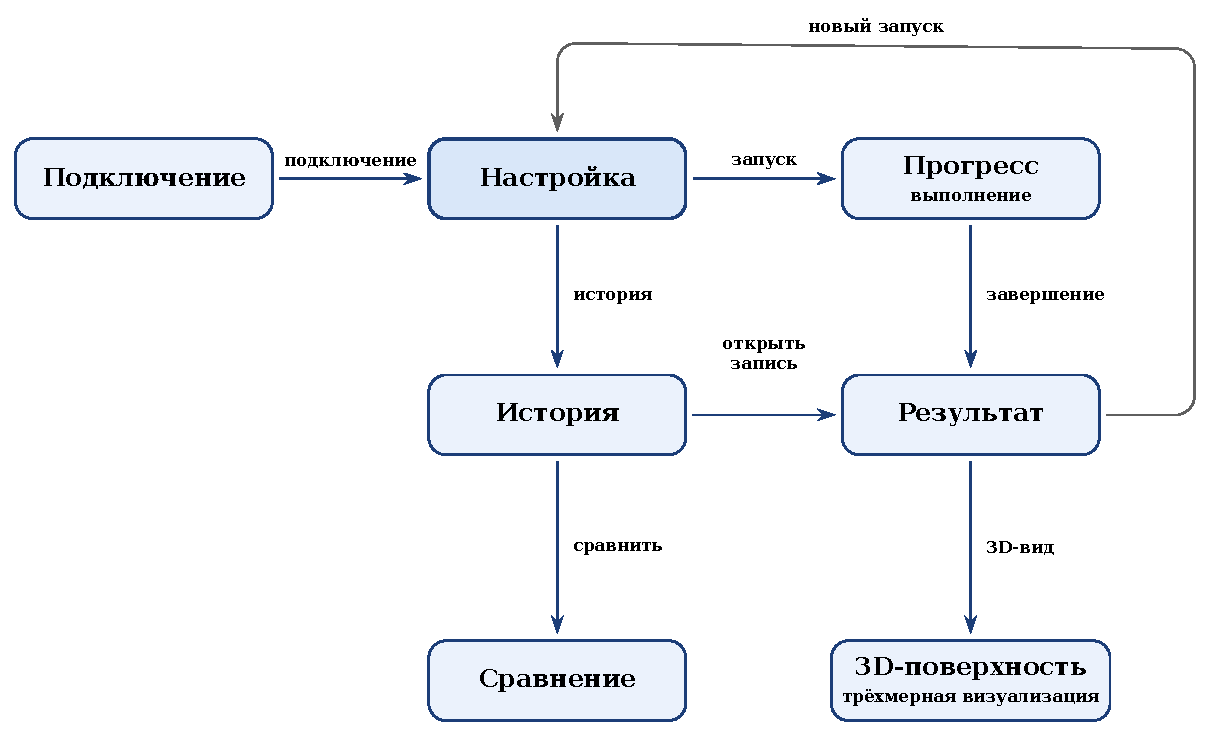
\includegraphics[width=0.95\linewidth]{navigation.pdf}
  \caption{Схема навигации между экранами приложения}
  \label{fig:navigation}
\end{figure}

Работа начинается с экрана подключения, на котором задаётся адрес сервера и
устанавливается соединение. После успешного подключения пользователь попадает на
экран настройки --- центральный экран приложения. Здесь выбирается метод
оптимизации, задаётся целевая функция, размерность и границы области поиска, а
также параметры выбранного метода. С этого же экрана можно перейти к истории
прошлых экспериментов.

После запуска эксперимента открывается экран прогресса. На нём отображается номер
текущего поколения, лучшее найденное значение и график сходимости, который
обновляется в реальном времени по мере поступления данных с сервера. Когда
вычисление завершается, приложение переходит на экран результата.

Экран результата показывает итог запуска: лучшее найденное решение, числовые
показатели и график сходимости за весь запуск, а также визуализацию пространства
поиска в виде контурной карты. С него можно открыть отдельный экран с трёхмерной
поверхностью целевой функции, вернуться к настройке для нового запуска или
перейти к истории. Завершённый эксперимент при этом сохраняется в историю.

Экран истории содержит список ранее проведённых экспериментов. Любую запись из
него можно открыть, чтобы снова увидеть её результат, а отметив несколько записей,
перейти к их сравнению. На экране сравнения результаты нескольких запусков
выводятся вместе: на совмещённом графике сходимости, в виде таблицы показателей и
столбчатой диаграммы. Такое разделение на экраны даёт простой и предсказуемый путь
от постановки задачи до анализа и сравнения результатов.

% =====================================================================
%  3. ТЕХНОЛОГИЧЕСКАЯ ЧАСТЬ
% =====================================================================
\section{Технологическая часть}\label{sec:technology}

\subsection{Обоснование выбора технологий}
\label{subsec:stack}

Архитектура, описанная в конструкторской части, не привязана к конкретным
технологиям. В этом подразделе обосновывается выбор средств, которыми
комплекс реализован: транспортного протокола, серверного и клиентского
языков, модели параллельной обработки и формата обмена данными.

Транспортный протокол должен удовлетворять трём условиям. Сервер обязан
отправлять данные клиенту по собственной инициативе, после каждого поколения и
не дожидаясь запроса. Соединение должно оставаться открытым всё время работы
задачи. Накладные расходы на сообщение должны быть малыми, поскольку сообщения о
прогрессе идут потоком --- по одному на поколение. Этим условиям отвечают не все
распространённые решения. Классический обмен по протоколу HTTP с периодическим
опросом сервера прост, но неэффективен: большинство запросов возвращают пустой
ответ, а интервал опроса задаёт минимальную задержку между появлением данных и их
получением~\cite{olifer2016}. Технология однонаправленной потоковой передачи
событий от сервера снимает проблему опроса, но не поддерживает обратную связь:
клиент не может по тому же соединению отправить задачу или команду отмены. Всем
трём условиям отвечает протокол WebSocket. Он устанавливает постоянное
двустороннее соединение поверх TCP, по которому обе стороны шлют сообщения в любой
момент, а заголовок каждого кадра занимает лишь несколько байт~\cite{fedulov2025}.
Поэтому в качестве транспорта выбран WebSocket.

Серверная часть написана на языке Python. Он стал стандартным языком научных
вычислений во многом благодаря библиотеке NumPy~\cite{numpy2020}, которая обеспечивает быстрые
операции над многомерными массивами~\cite{yavorski2024}. Операции над всей
популяцией --- вычисление целевой функции для всех особей, сортировка, отбор
доноров --- выражаются через действия над массивами NumPy и выполняются на уровне
скомпилированного кода, что значительно быстрее эквивалентных циклов на чистом
Python.

Сервер должен обслуживать несколько клиентов одновременно, не останавливая работу
с одним из них на время вычислений для другого. Для этого применяется асинхронная
модель Python на основе библиотеки \texttt{asyncio}: множество соединений
обслуживаются в одном потоке за счёт того, что операция, ожидающая данных по сети,
уступает управление другим~\cite{yavorski2024}. Однако сам алгоритм оптимизации
вычислительно нагружен и не имеет точек ожидания, поэтому при запуске прямо в цикле
событий он заблокировал бы все остальные соединения. Чтобы этого избежать,
алгоритм запускается в отдельном потоке из пула потоков, а данные о прогрессе
передаются из него обратно в цикл событий через потокобезопасную очередь.
Веб-часть сервера построена на фреймворке FastAPI, который поддерживает соединения
WebSocket и работает поверх той же асинхронной модели~\cite{fastapi_docs}.

Сообщения протокола сериализуются в формате JSON. Этот формат поддерживается без
дополнительных библиотек и в Python, и в Dart~\cite{pythonjson, dartconvert}, а
его текстовое представление удобно читать при отладке. Существуют и более
компактные двоичные форматы, но выигрыш от них здесь не определяющий: сообщения о
прогрессе содержат немного числовых полей, и затраты на их сериализацию
пренебрежимо малы по сравнению со временем самих вычислений~\cite{shulman2021}.
Для оценки объёма: финальная популяция размером $50 \times 10$ содержит 500 чисел,
что в JSON составляет около 5--7~КБ --- приемлемо для однократной передачи по
завершении задачи. В потоке прогресса массив популяции не передаётся: клиент
получает лишь номер поколения и лучшее значение.

Клиентская часть написана на языке Dart с использованием фреймворка Flutter. Dart
обладает строгой статической типизацией и встроенной поддержкой асинхронного
программирования~\cite{ryabokon2013}. Особенно важна абстракция потока асинхронных
событий: поток сообщений, приходящих по WebSocket, естественно представляется
такой последовательностью, на которую приложение подписывается и реагирует по мере
поступления данных. Flutter --- кроссплатформенный фреймворк, который компилирует
приложение в нативный код и использует собственный движок
рендеринга~\cite{kamyshev2020}. Интерфейс описывается деревом виджетов, и при
получении новых данных от сервера перестраивается только изменившаяся его часть,
что позволяет плавно обновлять график сходимости в реальном времени. Для рисования
контурной карты и трёхмерной поверхности используется низкоуровневый интерфейс
рисования на холсте, дающий доступ к отдельным графическим примитивам.

\subsection{Реализация вычислительного ядра сервера}
\label{subsec:core}

Вычислительное ядро сервера отвечает за запуск алгоритмов оптимизации. Оно
состоит из трёх частей: реестра методов, набора целевых функций и связующего
модуля запуска. Такое разделение позволяет добавлять новые алгоритмы и функции,
не меняя остальной код сервера.

Реестр методов --- это единая точка, в которой перечислены все доступные
алгоритмы. Каждому методу сопоставляется пара из класса алгоритма и класса его
конфигурации, а ключом служит строковое имя метода, которое приходит от клиента в
запросе на запуск. Содержимое реестра показано в листинге~\ref{lst:registry}.

\begin{lstlisting}[language=Python, caption={Реестр методов оптимизации}, label={lst:registry}]
METHODS = {
    "bbo.classic": (ClassicBBO, ClassicBBOConfig),
    "bbo.classic.modified": (ClassicBBO_Modified, BBOConfigModified),
    "bbo.sinusoidal": (BBO_Sinusoidal, SinBBOConfig),
    "bbo.sinusoidal.modified": (BBO_Sinusoidal_Modified, BBOConfigSinModified),
    "bbo.mixed": (BBO_Mixed, MixedBBOConfig),
    "bbo.mixed.modified": (BBO_Mixed_Modified, BBOConfigMixedModified),
    "pso": (PSO, PSOConfig),
}
\end{lstlisting}

Чтобы создать алгоритм, фабрика находит в реестре пару по имени метода, собирает
объект конфигурации из присланных параметров, дополняя его размерностью и
границами области, и возвращает готовый к запуску экземпляр алгоритма. Если имя
метода в реестре отсутствует, фабрика сообщает об ошибке. Благодаря этому
добавление нового алгоритма сводится к его регистрации в реестре --- остальной код
изменять не требуется.

Целевая функция создаётся отдельно. Система поддерживает два вида функций.
Встроенные функции --- сфера, Растригина, Экли и Букина~N.6 --- выбираются по
имени из заранее заданного набора. Кроме того, пользователь может задать свою
функцию в виде математического выражения от координат. Выполнять такое выражение
напрямую небезопасно: в нём может оказаться обращение к файловой системе или иной
нежелательный код. Поэтому выражение не вычисляется как обычный код, а сначала
разбирается в синтаксическое дерево, которое проверяется на допустимость. В
выражении разрешены только арифметические операции и функции из ограниченного
набора --- квадратный корень, экспонента, логарифм, тригонометрические функции и
подобные. Любой вызов постороннего имени или обращение к атрибуту объекта приводят
к отклонению выражения. Только прошедшее проверку выражение компилируется в
функцию. При вычислении ей доступны лишь координаты точки и функции из
разрешённого набора, а доступ к встроенным средствам языка закрыт, поэтому даже
если какая-то опасная конструкция минует проверку, выполнить её будет
нечем~\cite{yavorski2024}.

Связующий модуль запуска объединяет эти части и выполняет один запуск от начала до
конца. Он разбирает пришедшие параметры задачи, строит границы области поиска,
создаёт целевую функцию и алгоритм, после чего запускает оптимизацию. Во время
работы алгоритм вызывает переданную ему функцию обратного вызова после каждого
поколения; через неё модуль запуска передаёт данные о прогрессе наружу и
одновременно проверяет, не поступила ли команда отмены. Если отмена запрошена,
выполнение прерывается. По завершении модуль приводит результат к виду, пригодному
для передачи по сети: массивы значений преобразуются в списки, добавляются
сведения о затраченном времени и использованном методе.

\subsection{Реализация очереди задач и обработчика}
\label{subsec:queue}

Поскольку сервер может обслуживать несколько клиентов сразу, а каждый запуск
оптимизации занимает заметное время, задачи не выполняются немедленно по
поступлении, а проходят через очередь. За постановку задач в очередь и их
извлечение отвечает очередь задач, а за само выполнение --- обработчик.

Очередь реализована на основе приоритетной очереди из библиотеки \texttt{asyncio}.
Каждый элемент очереди --- это тройка из числового приоритета, порядкового номера
постановки и идентификатора задачи. Поддерживаются три уровня приоритета: высокий,
обычный и низкий; при равных приоритетах задачи выполняются в порядке поступления,
для чего и служит порядковый номер. Сам объект задачи хранится в отдельном
реестре, а в очереди лежит только его идентификатор, по которому обработчик
получает задачу целиком.

При постановке задачи очередь решает ещё две вспомогательные проблемы. Первая ---
защита от повторной постановки. Клиент присваивает каждому запросу уникальный
идентификатор; если из-за нестабильного соединения запрос придёт повторно, очередь
обнаружит совпадение по этому идентификатору и вернёт уже существующую задачу,
не создавая новую и не запуская повторных вычислений. Вторая --- защита от
переполнения: число одновременно ожидающих задач ограничено, и при достижении
предела новая постановка отклоняется с сообщением об ошибке. Кроме того, по
идентификатору задачи можно узнать её позицию в очереди и приблизительное время
ожидания, а также отменить задачу --- как ожидающую, так и уже выполняемую.

Выполнением задач занимается обработчик. Таких обработчиков несколько: при запуске
сервера создаётся пул из нескольких параллельных обработчиков, и их число задаётся
в настройках сервера. Каждый из них работает в постоянном цикле: извлекает из
очереди очередную задачу, переводит её в состояние выполнения, уведомляет клиента
о начале и запускает оптимизацию. Поскольку несколько обработчиков берут задачи из
общей очереди, сервер может выполнять сразу несколько задач одновременно. Сам
алгоритм оптимизации вычислительно нагружен и выполняется без точек ожидания,
поэтому его нельзя запускать прямо в асинхронном цикле событий --- это заблокировало
бы обработку остальных соединений. Поэтому алгоритм запускается в отдельном потоке
из пула, а асинхронный цикл тем временем продолжает обслуживать других
клиентов~\cite{yavorski2024}.

На время выполнения задаётся ограничение по времени. Запуск алгоритма обёрнут в
ожидание с таймаутом: если вычисление не завершилось за отведённый срок, оно
прерывается, а задача переходит в состояние превышения времени. Аналогично
обрабатываются и другие исходы --- успешное завершение, ошибка во время
вычислений и отмена пользователем; каждому из них соответствует свой переход в
терминальное состояние и своё сообщение клиенту.

Отдельного внимания заслуживает передача прогресса. Алгоритм выполняется в рабочем
потоке, а отправка сообщений клиенту идёт в асинхронном цикле, поэтому напрямую
передавать данные между ними нельзя. Прогресс переправляется через потокобезопасную
очередь: после каждого поколения рабочий поток помещает в неё данные, а отдельная
задача в цикле событий извлекает их и отправляет клиенту. Такая передача
поддерживает несколько режимов: сообщать о каждом поколении, о каждом $k$-м или не
сообщать вовсе, что позволяет снизить плотность потока сообщений для длительных
запусков. Когда вычисление завершается, в очередь прогресса помещается признак
конца, по которому отправка прогресса корректно останавливается.

Связь очереди с клиентами обеспечивает обработчик соединений. Для каждого
подключившегося клиента создаётся отдельный обработчик, который ведёт диалог с ним
по протоколу обмена. Сначала он принимает приветственное сообщение и в ответ
сообщает клиенту о возможностях сервера: какие методы оптимизации доступны, какие
виды целевых функций поддерживаются, какие есть режимы передачи прогресса и каков
предельный размер сообщения. Если первым приходит не приветствие, соединение
отклоняется. После рукопожатия обработчик входит в цикл чтения сообщений и
направляет каждое из них в зависимости от типа: запрос на запуск ставит задачу в
очередь, запрос на отмену снимает задачу, запрос состояния возвращает сведения о
задаче, а служебное сообщение проверки связи подтверждается ответом. Сообщения
неизвестного типа или с некорректными данными не прерывают работу --- в ответ
отправляется сообщение об ошибке, и обработчик продолжает принимать следующие.
Когда клиент отключается, обработчик отменяет все его незавершённые задачи, чтобы
сервер не тратил ресурсы на вычисления, результат которых уже некому получить.

Перед постановкой в очередь параметры задачи проверяются на корректность. Проверка
охватывает структуру сообщения и допустимость значений: имя метода должно быть
известным, размерность и размер популяции --- положительными, границы области ---
согласованными. Некорректный запрос отклоняется с понятным сообщением об ошибке
ещё до запуска вычислений, что защищает сервер от заведомо неверных задач.

\subsection{Реализация алгоритмов оптимизации}
\label{subsec:algo-impl}

Все семь методов реализованы по общей схеме. Каждый алгоритм оформлен как
отдельный класс, который получает при создании три вещи: конфигурацию, целевую
функцию и функцию обратного вызова для передачи прогресса. Основную работу
алгоритм выполняет в методе \texttt{optimize}: он инициализирует популяцию,
проводит заданное число поколений и возвращает результат --- лучшее решение, его
значение, историю сходимости и финальное состояние популяции. Различаются методы
тем, что происходит внутри одного поколения.

Параметры каждого метода описаны отдельным классом конфигурации. В нём заданы
значения по умолчанию и проверки корректности: например, размер популяции не
меньше двух, вероятность мутации лежит в отрезке от нуля до единицы, а число
элитных решений меньше размера популяции. Если границы области поиска не заданы
явно, они заполняются значениями по умолчанию. Эти проверки выполняются при
создании конфигурации, поэтому некорректные параметры отсекаются до запуска
вычислений. Случайность всех алгоритмов исходит из одного генератора, создаваемого
с заданным начальным значением, --- это делает запуски воспроизводимыми, что важно
при сравнении методов.

Рассмотрим реализацию классического BBO. Одно его поколение показано в
листинге~\ref{lst:bbo-gen}. Сначала популяция сортируется по значению целевой
функции, после чего по рангам вычисляются скорости эмиграции и иммиграции. Затем
для каждого неэлитного решения выполняется покомпонентная иммиграция: компонента
заменяется значением донора с вероятностью, равной скорости иммиграции, а донор
выбирается случайно с вероятностью, пропорциональной скорости эмиграции. После
миграции применяется мутация, а в конце поколения лучшие решения возвращаются в
популяцию вместо худших потомков.

\begin{lstlisting}[language=Python, caption={Одно поколение классического BBO}, label={lst:bbo-gen}]
order = np.argsort(fitness)
X, fitness = X[order], fitness[order]
best_f, best_x = float(fitness[0]), X[0].copy()

lambdas, mus = self._rank_based_migration_rates(self.cfg.pop_size)
donor_probs = lambdas[::-1] / lambdas[::-1].sum()
donor_cdf = np.cumsum(donor_probs)

Z = X.copy()
for k in range(self.cfg.elite_count, self.cfg.pop_size):
    imm_flags = self.rng.random(self.cfg.dims) < mus[::-1][k]
    for s in np.where(imm_flags)[0]:
        j = self._roulette_select(donor_cdf)
        Z[k, s] = X[j, s]
    mut_flags = self.rng.random(self.cfg.dims) < self.cfg.mutation_rate
    Z[k, mut_flags] = self.low[mut_flags] + self.rng.random(mut_flags.sum()) * self.span[mut_flags]

fit_Z = self._evaluate_population(self._clip(Z))
worst = np.argsort(fit_Z)[-self.cfg.elite_count:]
Z[worst], fit_Z[worst] = X[:self.cfg.elite_count], fitness[:self.cfg.elite_count]
X, fitness = Z, fit_Z
\end{lstlisting}

Варианты с синусоидальной и смешанной моделями миграции построены по тому же
циклу. Отличие у них только в одном месте --- в способе вычисления скоростей
$\lambda_r$ и $\mu_r$: каждый вариант рассчитывает их по своей формуле, приведённой
в подразделе~\ref{subsec:migration}. Всё остальное --- сортировка, покомпонентная
иммиграция, мутация, элитарность --- совпадает с классическим вариантом.

Модифицированные версии устроены сложнее. К базовому циклу в них добавлены три
механизма адаптации: мутации, частичный перезапуск и локальный поиск, и поколение
складывается из большего числа шагов. Его структура показана в
листинге~\ref{lst:bbo-mod}. В начале поколения вычисляется текущая вероятность
мутации, которая линейно убывает от начального значения к конечному. Затем
проверяется счётчик стагнации: если лучшее решение не улучшалось заданное число
поколений, выполняется частичный рестарт, а вероятность мутации временно
повышается. После этого идут миграция и мутация, применяется элитарность, и при
необходимости запускается локальный поиск. В конце поколения счётчик стагнации
обновляется в зависимости от того, удалось ли улучшить лучшее решение.

\begin{lstlisting}[language=Python, caption={Одно поколение модифицированного BBO}, label={lst:bbo-mod}]
mutation_rate = self._current_mutation_rate(gen)
if stagnation >= self.cfg.stagnation_generations:
    X, fit = self._restart_partially(X, fit)
    mutation_rate = min(self.cfg.mutation_start,
                        mutation_rate * self.cfg.mutation_boost_factor)
    stagnation = 0

X_new = self._migration_step(X, fit)
X_new = self._mutation_step(X_new, mutation_rate)
fit_new = self._evaluate(X_new)
X, fit = self._apply_elitism(X, fit, X_new, fit_new)

if self.cfg.enable_local_search and (gen + 1) % self.cfg.local_search_interval == 0:
    X, fit = self._local_search(X, fit, gen)

cur_best = float(fit[np.argmin(fit)])
if cur_best < best_f:
    best_f, stagnation = cur_best, 0
else:
    stagnation += 1
\end{lstlisting}

Частичный рестарт реализован как замена доли худших решений новыми случайными.
Число заменяемых решений определяется заданной долей от размера популяции, при этом
элитные решения защищены от замены. Локальный поиск уточняет несколько лучших
решений: к каждому из них последовательно добавляется случайное гауссовское
возмущение, масштаб которого пропорционален ширине области поиска и убывает с
номером поколения. Если возмущённая точка оказывается лучше, она принимается, иначе
отвергается. Так локальный поиск повышает точность вблизи найденных минимумов,
не затрагивая остальную популяцию.

Метод роя частиц реализован матрично: вся популяция обновляется за одну группу
операций над массивами, без цикла по частицам. Одна итерация PSO показана в
листинге~\ref{lst:pso-step}. Скорости всех частиц пересчитываются сразу: к
инерционной составляющей добавляются когнитивная, направленная к личному лучшему
положению, и социальная, направленная к глобально лучшему. Затем скорости
ограничиваются по модулю, положения сдвигаются и отсекаются по границам области,
после чего обновляются личные и глобально лучшее решения.

\begin{lstlisting}[language=Python, caption={Одна итерация метода роя частиц}, label={lst:pso-step}]
w = self._inertia_weight(t)
r1, r2 = self.rng.random((N, n)), self.rng.random((N, n))

cognitive = self.cfg.c1 * r1 * (pbest_pos - X)
social    = self.cfg.c2 * r2 * (gbest_pos - X)
V = w * V + cognitive + social
V = np.clip(V, -self.vmax, self.vmax)

X = np.clip(X + V, self.low, self.high)
fit = self._evaluate(X)

improved = fit < pbest_fit
pbest_pos[improved], pbest_fit[improved] = X[improved], fit[improved]
g_idx = int(np.argmin(pbest_fit))
if pbest_fit[g_idx] < gbest_fit:
    gbest_fit, gbest_pos = float(pbest_fit[g_idx]), pbest_pos[g_idx].copy()
\end{lstlisting}

Использование операций над массивами NumPy здесь принципиально. Вычисление целевой
функции сразу для всей популяции, сортировка, отбор и пересчёт скоростей
выполняются как единые операции над матрицами, а не как циклы на чистом
Python~\cite{yavorski2024}. Для метода роя частиц это позволяет полностью
избавиться от цикла по частицам; в BBO покомпонентная иммиграция всё же требует
перебора, поскольку для каждой компоненты донор выбирается независимо, но оценка
популяции и мутация остаются векторными. При вычислении целевой функции учитывается
её вид: сначала функция вызывается сразу для всей матрицы решений, и лишь если так
вычислить не удалось --- например, для пользовательского выражения, рассчитанного
поточечно, --- происходит переход к поэлементному вычислению. После каждого
поколения все методы вызывают функцию обратного вызова, передавая ей номер
поколения и лучшее найденное значение, --- именно эти данные затем уходят клиенту
в потоке прогресса.

\subsection{Реализация мобильного клиента}
\label{subsec:client-impl}

Мобильный клиент построен по слоистой схеме. Нижний слой отвечает за связь с
сервером по протоколу обмена, средний хранит состояние экранов и обрабатывает
события, верхний отображает интерфейс. Дополнительно выделены слой моделей данных,
описывающий структуру сообщений, и слой хранения, отвечающий за локальную базу
истории. Такое разделение позволяет менять одну часть, не затрагивая остальные.

\subsubsection{Клиент протокола}
Связь с сервером инкапсулирована в отдельном классе,
который скрывает детали соединения WebSocket и предоставляет приложению единый
поток событий. Сообщения от сервера разбираются и превращаются в типизированные
события, публикуемые в широковещательный поток; на него подписываются те части
приложения, которым нужны данные с сервера. Приём и маршрутизация сообщений
показаны в листинге~\ref{lst:ws-onmessage}: строка разбирается в конверт, из него
извлекаются тип и полезная нагрузка, после чего по типу создаётся соответствующее
событие.

\begin{lstlisting}[language=Dart, caption={Приём и маршрутизация сообщений на клиенте}, label={lst:ws-onmessage}]
void _onMessage(String raw) {
  final envelope = parseEnvelope(raw);
  final type = getType(envelope);
  final payload = getPayload(envelope);

  switch (type) {
    case MessageTypes.jobAccepted:
      _eventController.add(WsJobAccepted(JobAccepted.fromPayload(payload)));
    case MessageTypes.jobStarted:
      _eventController.add(WsJobStarted(JobStarted.fromPayload(payload)));
    case MessageTypes.jobProgress:
      _eventController.add(WsJobProgress(JobProgress.fromPayload(payload)));
    case MessageTypes.jobResult:
      _eventController.add(WsJobResult(JobResult.fromPayload(payload)));
    case MessageTypes.jobFinished:
      _eventController.add(WsJobFinished(JobFinished.fromPayload(payload)));
    case MessageTypes.error:
      _eventController.add(WsError(ProtocolError.fromPayload(payload)));
  }
}
\end{lstlisting}

Клиент протокола устойчив к обрывам связи. Если соединение неожиданно закрывается,
он пытается восстановить его автоматически, причём задержка между попытками растёт
по степенному закону --- от одной секунды до тридцати, --- чтобы не нагружать сеть
частыми попытками. Пока соединение установлено, клиент периодически посылает
служебное сообщение проверки связи. При подключении он отправляет серверу
приветствие, в котором сообщает о желании получать поток прогресса. Намеренное
отключение пользователем отличается от обрыва специальным признаком: при нём
автоматическое восстановление не запускается. Кроме приёма событий клиент
предоставляет методы для отправки задачи, запроса её состояния и отмены.

\subsubsection{Модели данных и конверт сообщения}
Сообщения протокола разбираются и
собираются в отдельном слое моделей. Каждому типу сообщения соответствует свой
класс с методом разбора из полезной нагрузки, благодаря чему остальной код работает
с типизированными объектами, а не с необработанными словарями. Формирование
исходящих сообщений вынесено в общую функцию построения конверта, которая
добавляет служебные поля заголовка --- версию протокола, тип, уникальный
идентификатор сообщения, метку времени и поля для связи сообщений и идентификации
задачи. Эта функция показана в листинге~\ref{lst:envelope}.

\begin{lstlisting}[language=Dart, caption={Построение конверта исходящего сообщения}, label={lst:envelope}]
Map<String, dynamic> buildEnvelope({
  required String type,
  required Map<String, dynamic> payload,
  String? clientReqId,
  String? jobId,
}) {
  return {
    'header': {
      'v': 1,
      'type': type,
      'msg_id': _uuid.v4(),
      'ts': DateTime.now().toUtc().toIso8601String(),
      'trace': {'client_req_id': clientReqId, 'job_id': jobId},
    },
    'payload': payload,
  };
}
\end{lstlisting}

\subsubsection{Сборка конфигурации задачи}
Параметры эксперимента, задаваемые на
экране настройки, собираются из нескольких независимых частей: описания целевой
функции, постановки задачи, выбранного метода, режима потоковой передачи и состава
выходных данных. Описание целевой функции хранит её вид --- встроенная или
заданная выражением --- и соответствующие поля. Постановка задачи задаёт
размерность и границы области поиска, которые могут быть едиными для всех
координат или различаться по каждой. Параметры метода зависят от выбранного
алгоритма: у каждого метода свой набор полей, например размер популяции и
вероятность мутации для BBO или коэффициенты для метода роя частиц. Каждая часть
умеет преобразовывать себя в представление для передачи, а перед отправкой все
части объединяются в единую полезную нагрузку запроса на запуск. Так на клиенте
формируется тот самый запрос, который сервер затем разбирает и исполняет.

\subsubsection{Управление состоянием}
Средний слой реализован по схеме
однонаправленного потока данных: каждому экрану соответствует объект управления
состоянием, который подписывается на поток событий клиента протокола, обрабатывает
их и порождает новое неизменяемое состояние, на которое реагирует интерфейс.
Таких объектов несколько: один отвечает за подключение к серверу, другой --- за
сборку конфигурации, третий --- за наблюдение за ходом задачи, четвёртый --- за
работу с историей. Наиболее показателен объект состояния экрана прогресса. При
создании он отправляет серверу задачу и подписывается на события, а получая
сообщения о ходе вычисления, инкрементально накапливает историю лучших значений,
как показано в листинге~\ref{lst:progress-cubit}. Новые значения дописываются в
конец уже накопленной истории, что и позволяет графику сходимости достраиваться в
реальном времени, не перестраиваясь заново.

\begin{lstlisting}[language=Dart, caption={Накопление истории прогресса}, label={lst:progress-cubit}]
case WsJobProgress(:final data):
  final newHistory = List<double>.from(state.historyBestF);
  if (data.progress.historyBestFTail != null) {
    for (final v in data.progress.historyBestFTail!) {
      if (newHistory.isEmpty || newHistory.last != v) newHistory.add(v);
    }
  } else {
    newHistory.add(data.progress.bestF);
  }
  emit(state.copyWith(
    phase: JobPhase.running,
    iteration: data.progress.iteration,
    bestF: data.progress.bestF,
    historyBestF: newHistory,
  ));
\end{lstlisting}

Этот же объект отслеживает фазу задачи: ожидание в очереди, начало выполнения, ход
вычисления и завершение. Когда от сервера приходит сообщение о завершении, фаза
переключается в одно из конечных состояний --- успех, ошибка, отмена или
превышение времени, --- и интерфейс соответственно меняет вид. Отдельно
накапливается история лучших решений в пространстве, которая затем используется
для построения траектории на трёхмерной визуализации.

\subsubsection{Локальное хранение истории}
История завершённых экспериментов хранится
на устройстве в локальной базе данных. Результат каждого запуска сериализуется в
текстовое представление и сохраняется отдельной записью вместе с метаданными ---
методом, целевой функцией, размерностью, итоговым значением и временем проведения.
При открытии истории записи считываются обратно и восстанавливаются в типизированные
объекты, а метаданные позволяют отбирать и фильтровать запуски. Хранение на самом
устройстве делает историю доступной независимо от того, подключён ли клиент к
серверу.

\subsection{Пользовательский интерфейс приложения}
\label{subsec:ui-impl}

В этом подразделе показано, как выглядит готовое приложение. Интерфейс выдержан в
едином стиле: общая цветовая гамма, крупные элементы управления, удобные для
работы на сенсорном экране, и привычные для мобильных приложений компоненты ---
выпадающие списки, переключатели и ползунки. Экраны рассматриваются в том порядке,
в каком пользователь обычно проходит через них при работе.

\subsubsection{Подключение к серверу}

С этого экрана начинается работа. Пользователь вводит адрес и порт сервера и
нажимает кнопку подключения; под кнопкой отображается текущее состояние
соединения. Адрес последнего использованного сервера сохраняется, поэтому при
повторном запуске его не нужно вводить заново. Экран подключения показан на
рисунке~\ref{fig:screen-connection}.

\begin{figure}[H]
  \centering
  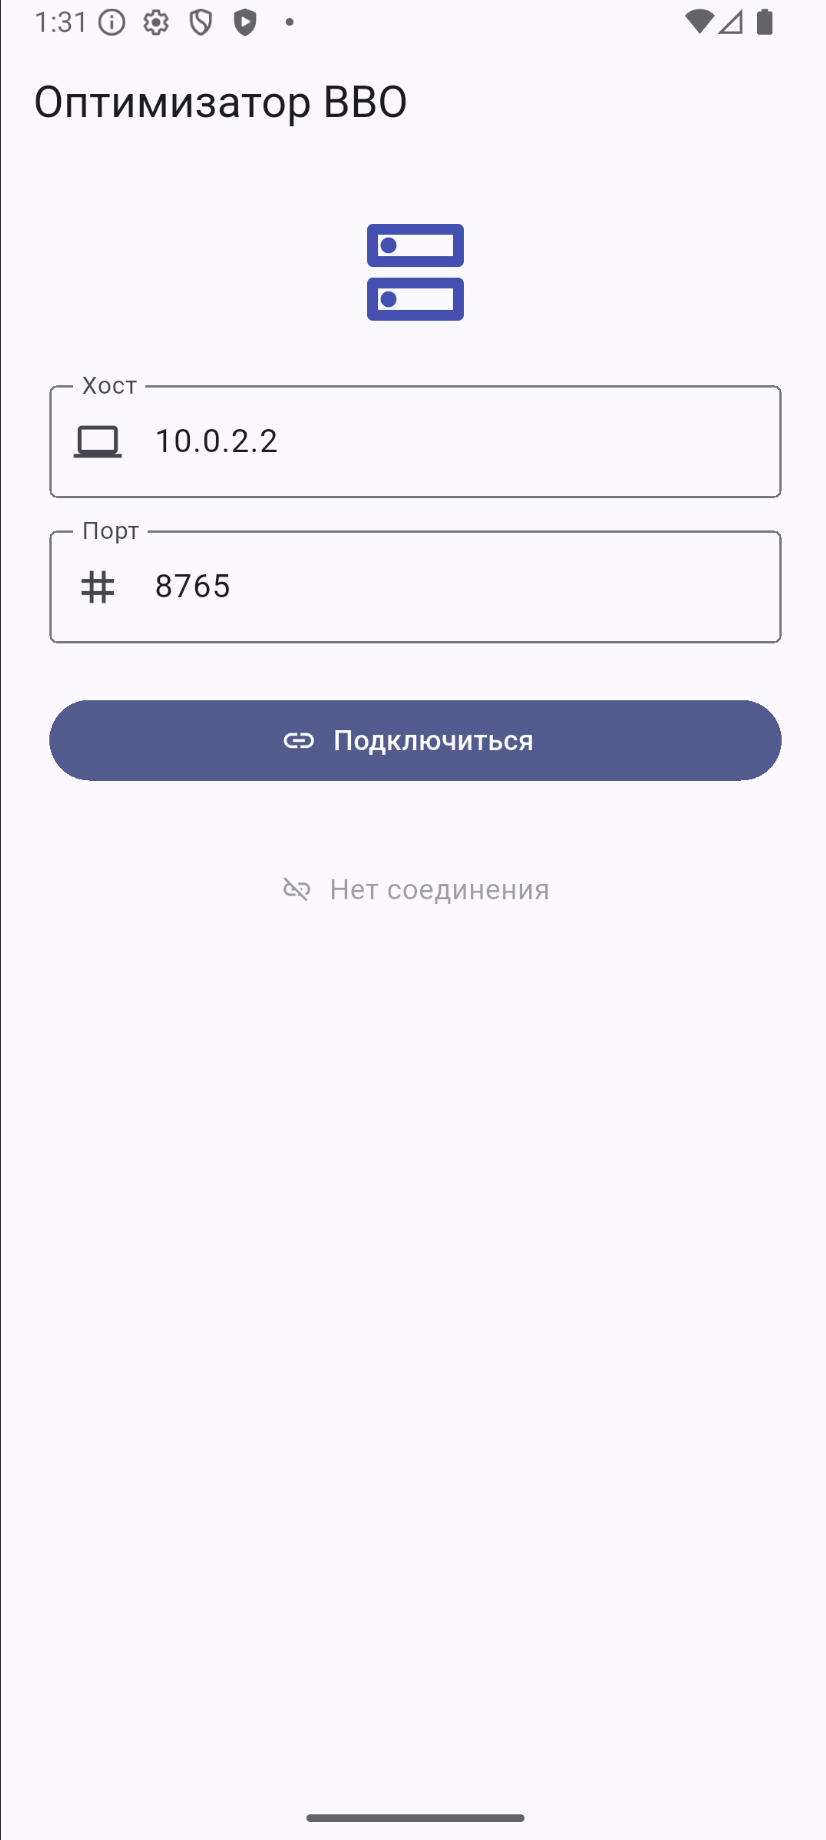
\includegraphics[width=0.4\linewidth]{screens/screen_connection.png}
  \caption{Экран подключения к серверу}
  \label{fig:screen-connection}
\end{figure}

\subsubsection{Настройка эксперимента}

После подключения открывается основной экран настройки. Он разбит на смысловые
блоки: выбор целевой функции, постановка задачи, метод оптимизации, режим
потоковой передачи и состав выходных данных. В блоке целевой функции выбирается
встроенная функция или вводится своё выражение, а переключатель задаёт минимизацию
или максимизацию. В блоке постановки задачи ползунком задаётся размерность, а в
полях ниже --- границы области поиска. В блоке метода выбирается алгоритм, и для
него появляется свой набор параметров: размер популяции, число поколений,
вероятность мутации и другие. Поскольку настроек много, экран прокручивается;
внизу находится кнопка запуска оптимизации. Вид экрана показан на
рисунке~\ref{fig:screen-config}.

\begin{figure}[H]
  \centering
  \begin{minipage}{0.4\linewidth}\centering
    
\includegraphics[width=\linewidth]{screens/screen_config1.png}
  \end{minipage}\hfill
  \begin{minipage}{0.4\linewidth}\centering
    
\includegraphics[width=\linewidth]{screens/screen_config2.png}
  \end{minipage}
  \caption{Экран настройки эксперимента: выбор функции и задачи (слева), параметры
  метода и потоковой передачи (справа)}
  \label{fig:screen-config}
\end{figure}

\subsubsection{Выполнение и наблюдение за прогрессом}

После запуска приложение переходит на экран выполнения. Вверху находится индикатор
прогресса с номером текущего поколения и долей выполнения, ниже --- лучшее
найденное значение и затраченное время. Основную часть экрана занимает график
сходимости, который достраивается в реальном времени по мере поступления данных с
сервера. Внизу расположена кнопка отмены, позволяющая прервать вычисление, не
дожидаясь его окончания. Экран выполнения показан на
рисунке~\ref{fig:screen-progress}.

\begin{figure}[H]
  \centering
  
\includegraphics[width=0.4\linewidth]{screens/screen_progress.png}
  \caption{Экран выполнения с графиком сходимости в реальном времени}
  \label{fig:screen-progress}
\end{figure}

\subsubsection{Просмотр результата}

По завершении вычисления открывается экран результата. Вверху выводится лучшее
найденное значение целевой функции, ниже --- координаты лучшего решения и сводка
показателей: метод, число поколений и вычислений функции, затраченное время. Далее
расположен график сходимости за весь запуск, а под ним --- визуализация
пространства поиска в виде контурной карты, на которой отмечены лучшее решение и
ближайшие к нему особи. Здесь же находятся кнопки построения анимации и перехода к
трёхмерной визуализации. Вид экрана показан на рисунке~\ref{fig:screen-results}.

\begin{figure}[H]
  \centering
  \begin{minipage}{0.3\linewidth}\centering
    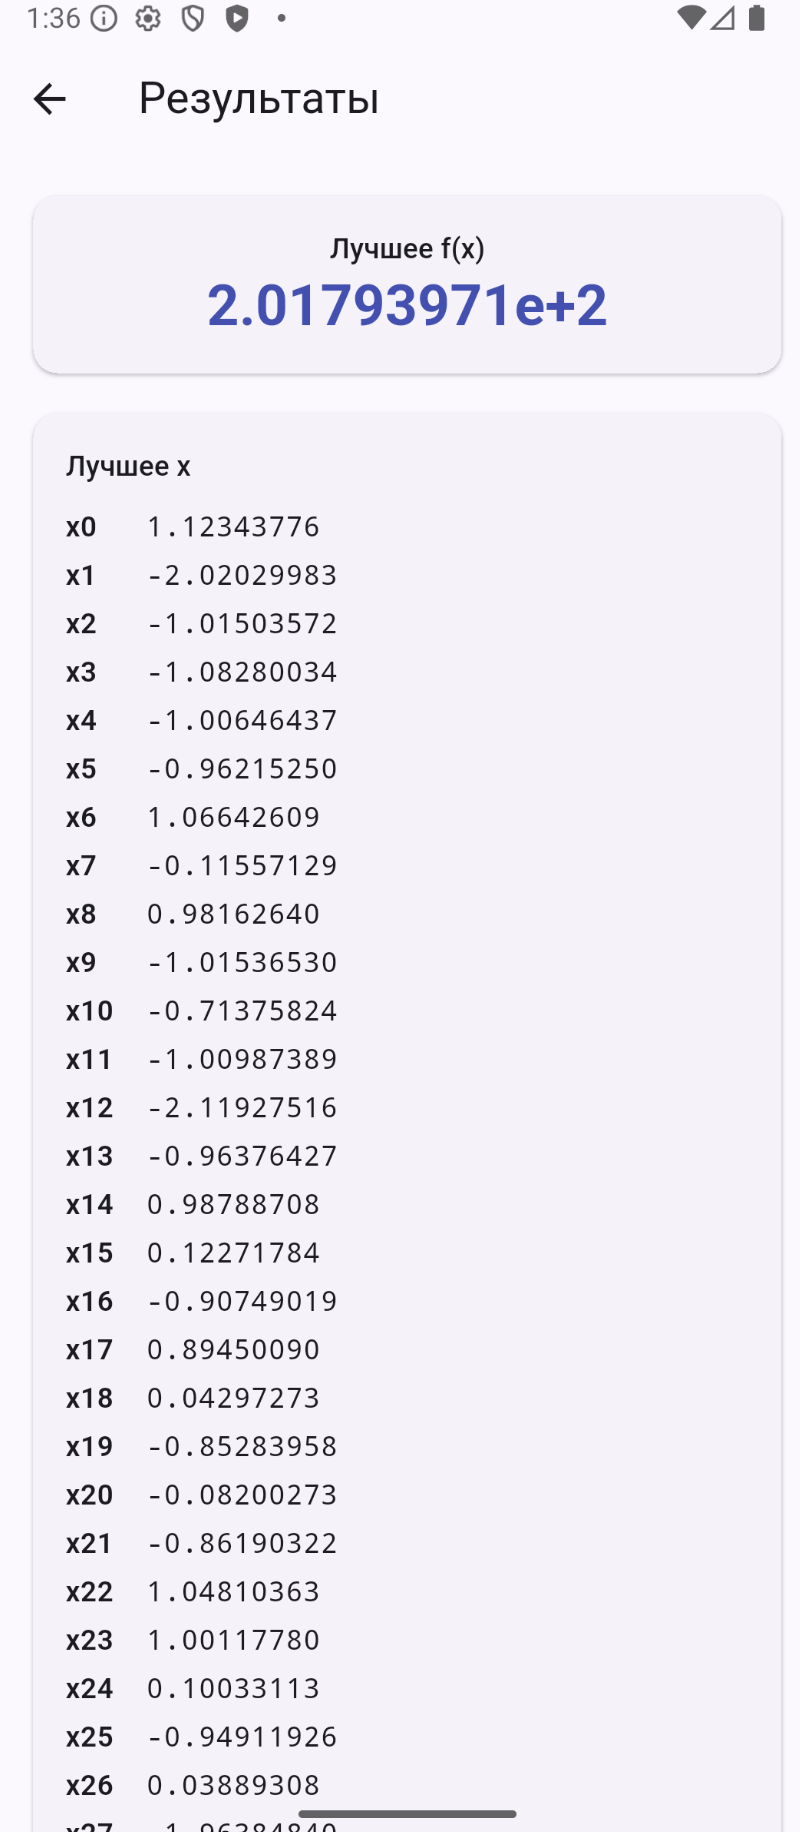
\includegraphics[width=\linewidth]{screens/screen_results1.png}
  \end{minipage}\hfill
  \begin{minipage}{0.3\linewidth}\centering
    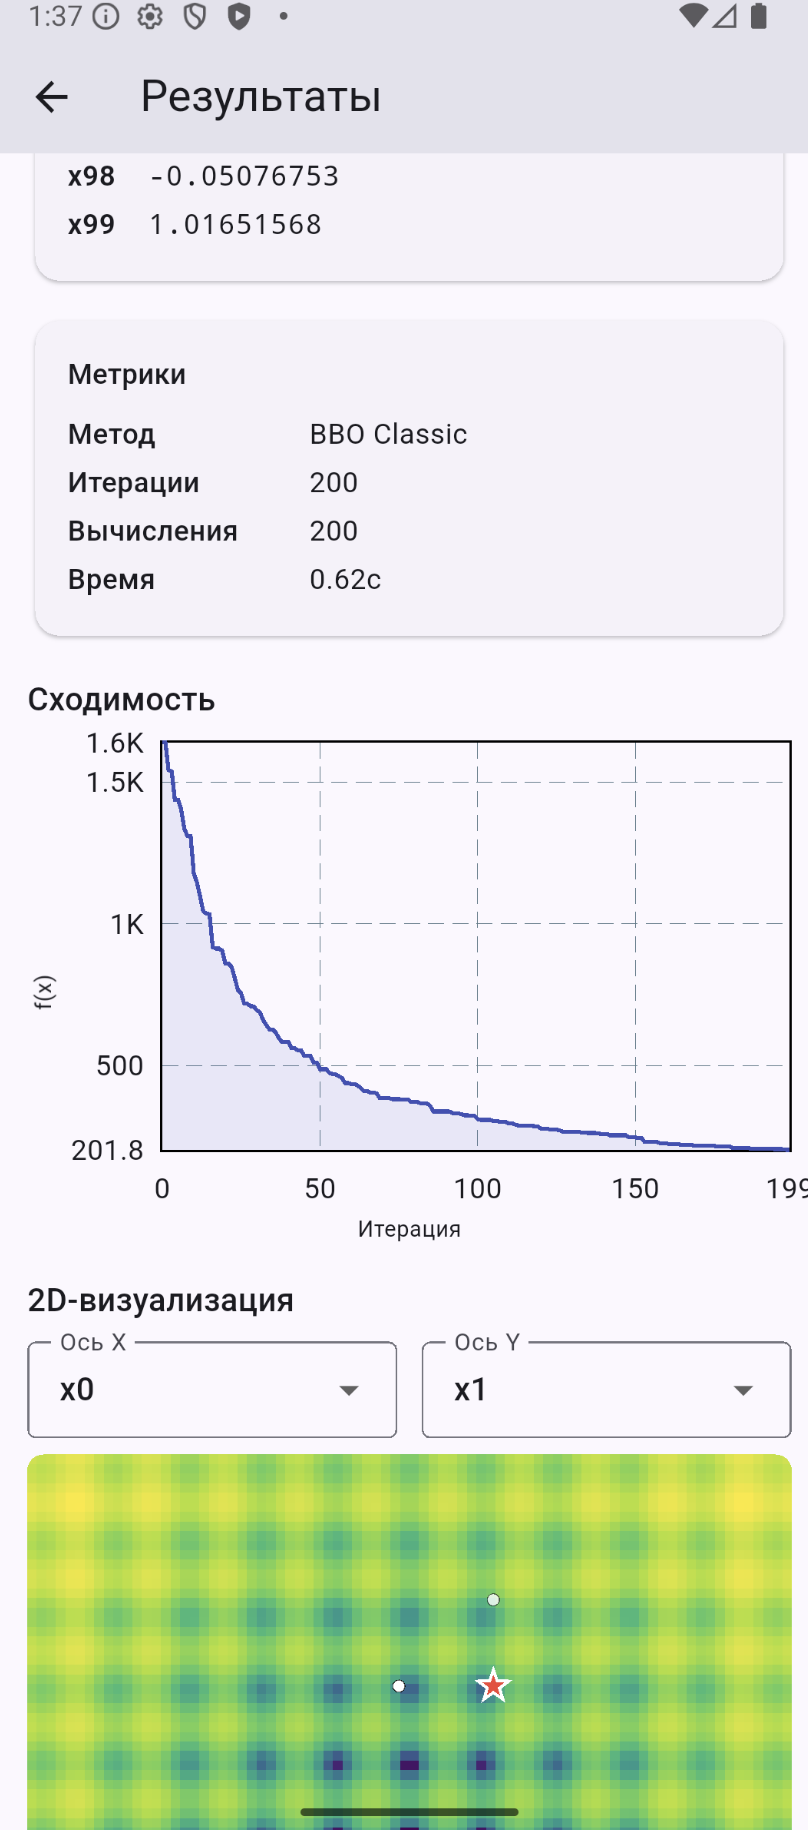
\includegraphics[width=\linewidth]{screens/screen_results2.png}
  \end{minipage}\hfill
  \begin{minipage}{0.3\linewidth}\centering
    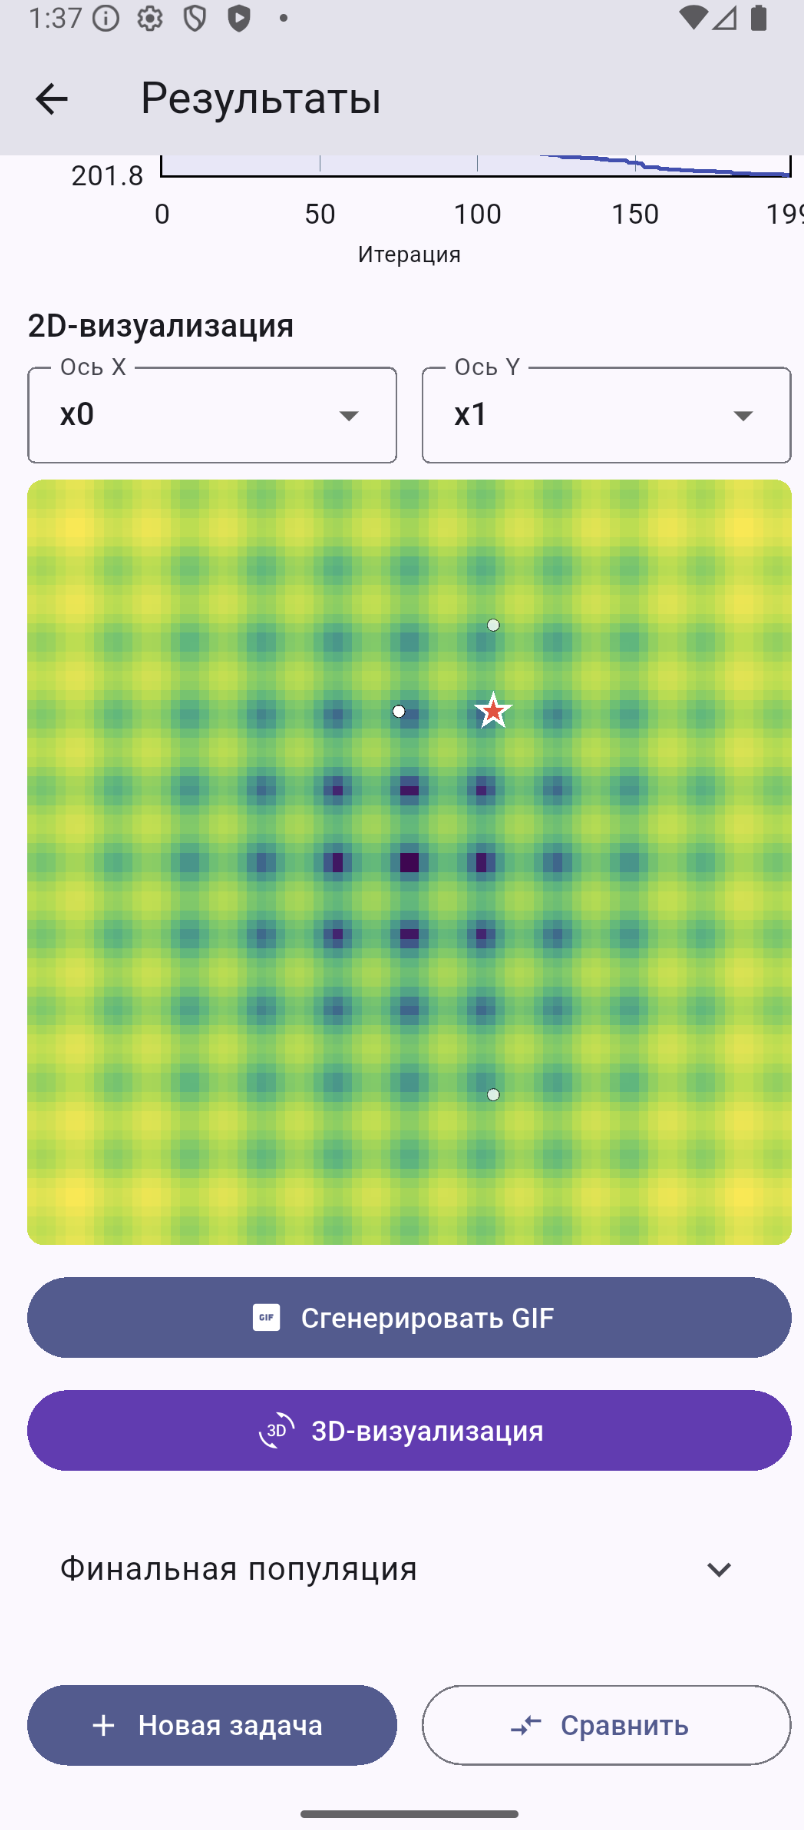
\includegraphics[width=\linewidth]{screens/screen_results3.png}
  \end{minipage}
  \caption{Экран результата: лучшее решение (слева), показатели и график сходимости (в центре), контурная
  карта пространства поиска (справа)}
  \label{fig:screen-results}
\end{figure}

По нажатию кнопки строится анимация: контурная карта, на которой популяция
смещается от поколения к поколению. Готовая анимация показывается прямо на экране,
как на рисунке~\ref{fig:screen-gif}.

\begin{figure}[H]
  \centering
  
\includegraphics[width=0.4\linewidth]{screens/screen_gif.png}
  \caption{Анимация процесса оптимизации на экране результата}
  \label{fig:screen-gif}
\end{figure}

\subsubsection{Трёхмерная визуализация}

Отдельный экран показывает целевую функцию трёхмерной поверхностью. Высота точки
соответствует значению функции, на поверхности отмечены лучшее решение и путь, по
которому оно улучшалось. Поверхность можно вращать движением пальца, рассматривая
рельеф под разными углами, а выпадающие списки сверху позволяют выбрать, какие две
координаты отложить по осям. Экран трёхмерной визуализации показан на
рисунке~\ref{fig:screen-3d}.

\begin{figure}[H]
  \centering
  
\includegraphics[width=0.4\linewidth]{screens/screen_3d.png}
  \caption{Экран трёхмерной визуализации целевой функции}
  \label{fig:screen-3d}
\end{figure}

\subsubsection{История и сравнение запусков}

Все завершённые эксперименты попадают в историю. На её экране они показаны списком,
где для каждого запуска указаны метод, целевая функция, размерность, итоговое
значение и время проведения; список можно фильтровать по методу и функции. Отметив
несколько запусков, пользователь переходит к их сравнению. На экране сравнения
выводятся совмещённый график сходимости выбранных запусков, таблица их показателей
и столбчатая диаграмма лучших значений. Оба экрана показаны на
рисунке~\ref{fig:screen-history}.

\begin{figure}[H]
  \centering
  \begin{minipage}{0.4\linewidth}\centering
    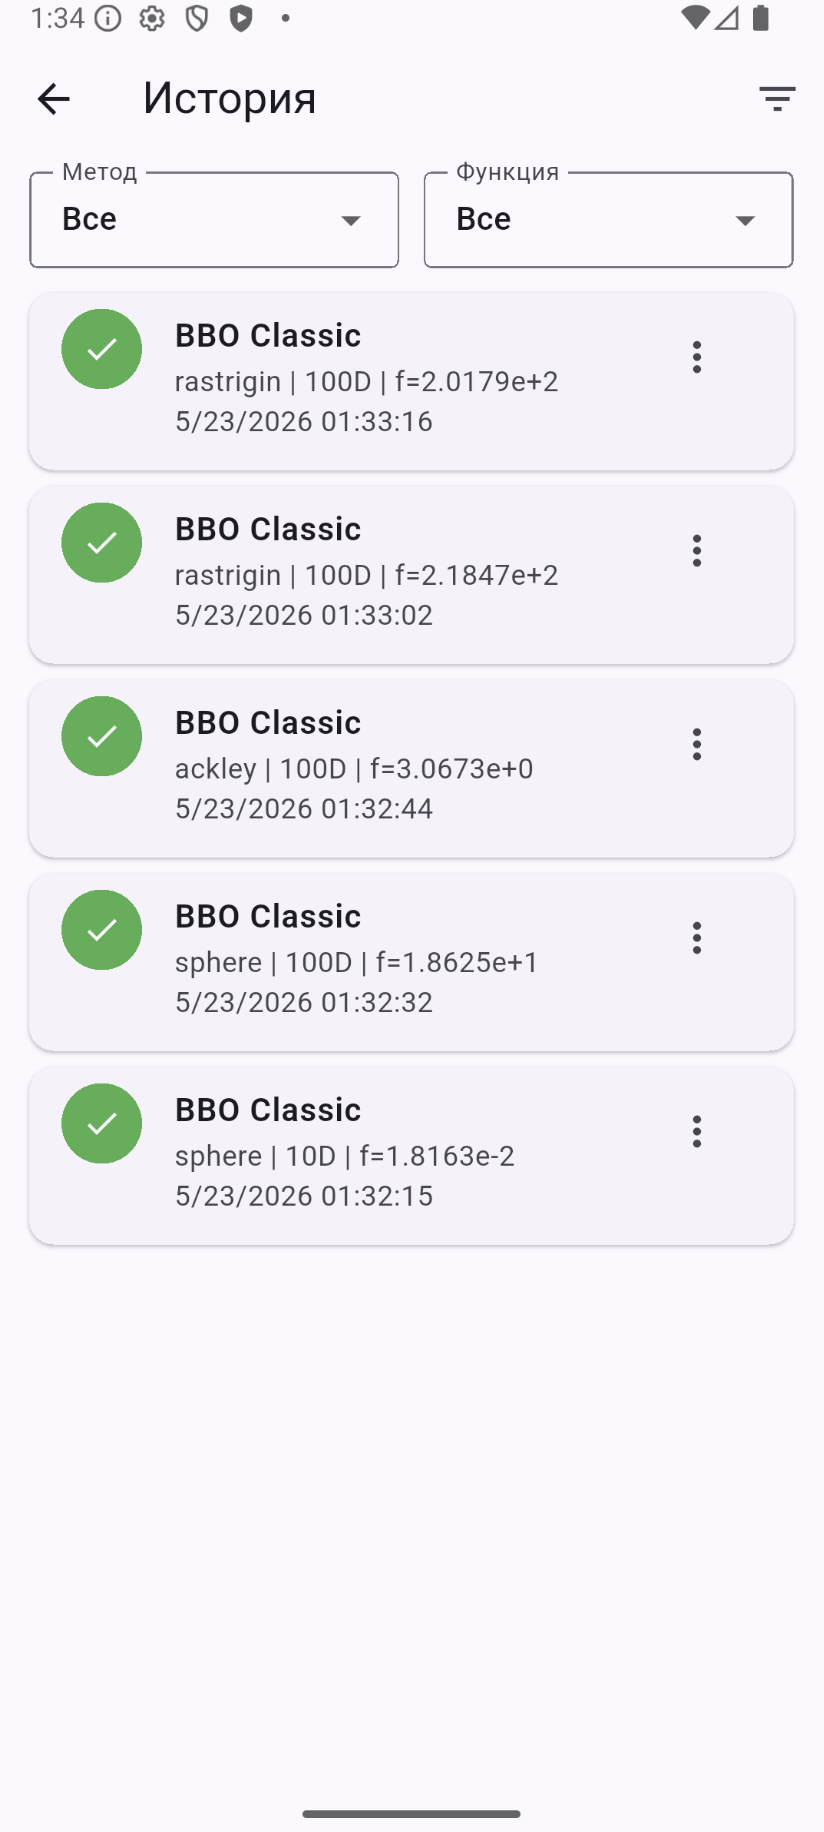
\includegraphics[width=\linewidth]{screens/screen_history.png}
  \end{minipage}\hfill
  \begin{minipage}{0.4\linewidth}\centering
    
\includegraphics[width=\linewidth]{screens/screen_comparison.png}
  \end{minipage}
  \caption{Экран истории экспериментов (слева) и экран сравнения запусков (справа)}
  \label{fig:screen-history}
\end{figure}

\subsection{Реализация визуализации результатов}
\label{subsec:visual-impl}

Способы визуализации реализованы на стороне клиента. График сходимости строится готовым средством
построения графиков, а контурная карта, трёхмерная поверхность и кадры анимации
рисуются вручную через низкоуровневый интерфейс рисования на холсте, который даёт
доступ к отдельным графическим примитивам. Ниже рассмотрена реализация каждого
вида.

\subsubsection{График сходимости}

График сходимости показывает, как убывает лучшее найденное значение от поколения к
поколению. Он строится готовым средством построения графиков, которому передаётся
список накопленных значений. На экране выполнения этот список пополняется по мере
прихода сообщений о прогрессе, поэтому график достраивается в реальном времени.
Когда значения функции убывают на несколько порядков, по оси ординат применяется
логарифмическая шкала, иначе нижняя часть кривой сжимается у нуля и становится
нечитаемой. На экране результата и на экране сравнения тот же график строится по
полной истории запуска, причём при сравнении на одни оси накладывается несколько
кривых, различающихся цветом.

\subsubsection{Контурная карта}

Контурная карта строится вручную. Область поиска разбивается на равномерную сетку,
для каждой ячейки вычисляется значение целевой функции, которое переводится в цвет
по выбранной цветовой шкале, и ячейка закрашивается прямоугольником. Значение
переводится в цвет через логарифмическую нормировку, что делает различимыми и
глубокие минимумы, и пологие участки. Поверх карты наносятся положения особей
популяции и отдельно отмечается лучшее решение. Основная часть рисования показана в
листинге~\ref{lst:contour}.

\begin{lstlisting}[language=Dart, caption={Построение контурной карты}, label={lst:contour}]
for (int j = 0; j < resolution; j++) {
  for (int i = 0; i < resolution; i++) {
    final val = grid.values[j][i];
    final t = range > 0
        ? (math.log(val - minVal + 1) / math.log(range + 1)).clamp(0.0, 1.0)
        : 0.0;
    paint.color = ColorMaps.viridis(t);
    canvas.drawRect(
      Rect.fromLTWH(i * cellW, j * cellH, cellW + 0.5, cellH + 0.5),
      paint,
    );
  }
}
\end{lstlisting}

Поскольку построение карты требует вычислить функцию во всех узлах сетки, оно
выполняется один раз при открытии экрана, а при перерисовке используются уже
полученные значения. При размерности задачи больше двух по осям откладываются две
выбранные пользователем координаты, а остальные фиксируются, что даёт сечение
функции в выбранной плоскости.

\subsubsection{Трёхмерная поверхность}

Трёхмерная поверхность строится по той же сетке значений функции. Узлы сетки
образуют четырёхугольные грани, которые проектируются на плоскость экрана. Проекция
выполняется по формулам поворота: координаты каждого узла нормируются к
единому диапазону и последовательно поворачиваются вокруг вертикальной и
горизонтальной осей, после чего две полученные координаты дают положение точки на
экране. Реализация проекции показана в листинге~\ref{lst:project}.

\begin{lstlisting}[language=Dart, caption={Проекция точки поверхности на экран}, label={lst:project}]
Offset project(double px, double py, double pz) {
  final nx = 2 * (px - xMin) / (xMax - xMin) - 1;
  final ny = 2 * (py - yMin) / (yMax - yMin) - 1;
  final nz = 2 * (pz - fMin) / fRange - 1;

  final rx = nx * cosZ - ny * sinZ;       // rotate around Z
  final ry = nx * sinZ + ny * cosZ;
  final ry2 = ry * cosX - nz * sinX;      // rotate around X

  return Offset(cx + rx * scale, cy - ry2 * scale);
}
\end{lstlisting}

Чтобы ближние грани правильно перекрывали дальние, применяется алгоритм художника:
для каждой грани вычисляется её глубина, грани сортируются от дальних к ближним и
рисуются в этом порядке. Цвет грани определяется средним значением функции в её
узлах по той же шкале, что и контурная карта. Поверх поверхности наносится путь
лучшего решения --- накопленная за время поиска последовательность точек,
соединённых линией; чтобы не рисовать тысячи точек, путь прореживается. Углы
поворота меняются жестом пользователя по экрану, и при каждом изменении поверхность
проектируется заново, благодаря чему её можно рассматривать под любым углом.

\subsubsection{Анимация процесса оптимизации}

Анимация показывает, как популяция смещалась от поколения к поколению. Она
собирается покадрово в формат GIF. Сначала строится фоновый кадр с контурной картой
целевой функции, затем для каждого кадра поверх фона наносятся положения особей и
лучшее решение, а также служебная строка с номером поколения и текущим лучшим
значением. Число кадров фиксировано, поэтому из всей истории берётся равномерная
выборка поколений. Готовые кадры собираются в один файл с заданной частотой смены,
причём последний кадр показывается дольше остальных, чтобы итоговое расположение
популяции было видно. Сборка кадров показана в листинге~\ref{lst:gif}.

\begin{lstlisting}[language=Dart, caption={Покадровая сборка анимации}, label={lst:gif}]
final step = math.max(1, totalIterations ~/ frameCount);
for (int f = 0; f < frameCount; f++) {
  final iterIndex = math.min(f * step, totalIterations - 1);
  final progress = (f + 1) / frameCount;
  final frame = img.Image.from(bgFrame);

  final visibleCount =
      (population.length * progress).round().clamp(1, population.length);
  for (int p = 0; p < visibleCount; p++) {
    final px = _mapCoord(population[p][dimX], xMin, xMax, size);
    final py = _mapCoord(population[p][dimY], yMin, yMax, size);
    _drawDot(frame, px, py, 2, img.ColorRgba8(255, 255, 255, 200));
  }
  _drawStar(frame, bx, by, starSize, img.ColorRgba8(255, 0, 0, 255));
  _drawInfoBar(frame, iterIndex, historyBestF[iterIndex], size);
  frames.add(frame);
}
\end{lstlisting}

Готовая анимация показывается прямо на экране результата и может быть сохранена как
обычный файл изображения. Поскольку формат GIF не требует внешних средств
воспроизведения и собирается из готовых кадров, он удобен для этой задачи.
\label{subsec:visualization}


% =====================================================================
%  ЗАКЛЮЧЕНИЕ — ~1 страница, не нумеруется
% =====================================================================
\structelem{ЗАКЛЮЧЕНИЕ}

В ходе выполнения работы был разработан программный комплекс для исследования и
визуализации модификаций алгоритма биогеографической оптимизации. Поставленная во
введении цель достигнута, а все связанные с ней задачи решены.

Реализовано серверное вычислительное ядро, поддерживающее семейство из семи
методов: классический BBO, его варианты с синусоидальной и смешанной моделями
миграции, три их модификации с адаптивной мутацией, перезапуском при стагнации и
локальным поиском, а также метод роя частиц. Алгоритмы запускаются как на четырёх
встроенных тестовых функциях, так и на функции, заданной пользователем в виде
выражения, причём такое выражение перед вычислением проверяется на безопасность.

Разработан протокол обмена данными поверх постоянного соединения WebSocket. Он
поддерживает постановку задачи, передачу прогресса по поколениям в реальном
времени, выдачу итогового результата и отмену задачи, а очередь с приоритетами и
пул обработчиков позволяют серверу обслуживать несколько клиентов одновременно.

Создано мобильное приложение, через которое пользователь настраивает эксперимент,
отправляет задачу на сервер и следит за ходом вычислений. Приложение построено по
слоистой схеме, а связь с сервером и хранение истории вынесены в отдельные слои,
что упростило его разработку.

Реализованы средства визуализации, наглядно показывающие работу алгоритма: график
сходимости, который достраивается в реальном времени, контурная карта и
трёхмерная поверхность пространства поиска с возможностью вращения, а также
анимация, показывающая динамику популяции. Это позволяет не только увидеть
итоговый результат, но и проследить за самим процессом поиска.

Организовано хранение истории экспериментов на устройстве и их сравнение.
Сохранённые запуски можно сопоставлять на совмещённом графике сходимости, в
таблице показателей и на столбчатой диаграмме, что и составляет основное
назначение комплекса.

Комплекс допускает дальнейшее развитие. Семейство методов можно расширить другими
метаэвристиками, добавив их в реестр без изменения остального кода. Набор тестовых
функций можно дополнить, а заложенные в протокол, но пока не используемые
разбиение больших сообщений на части и сжатие --- задействовать при работе с
большими объёмами данных. 

% =====================================================================
%  СПИСОК ИСПОЛЬЗОВАННЫХ ИСТОЧНИКОВ — 15-20 наименований, ГОСТ 7.32
% =====================================================================
\clearpage
\phantomsection
\addcontentsline{toc}{section}{СПИСОК ИСПОЛЬЗОВАННЫХ ИСТОЧНИКОВ}
\begin{center}\large\bfseries СПИСОК ИСПОЛЬЗОВАННЫХ ИСТОЧНИКОВ\end{center}
\vspace{8pt}
\printbibliography[heading=none]

% =====================================================================
%  ПРИЛОЖЕНИЯ
% =====================================================================
\structelem{ПРИЛОЖЕНИЯ}

\vspace{4pt}
\begin{center}\large\bfseries ПРИЛОЖЕНИЕ А\end{center}
\begin{center}\normalsize\bfseries Руководство пользователя\end{center}
\vspace{8pt}

Руководство описывает работу с мобильным приложением комплекса --- от запуска
сервера до анализа результатов. Предполагается, что серверная часть уже запущена
и доступна по сети, а мобильное приложение установлено на устройство.

Перед началом работы необходимо запустить сервер на компьютере, доступном по сети.
Сервер начинает принимать подключения по указанному адресу и порту. После этого
работа ведётся через мобильное приложение в следующем порядке.

\begin{enumerate}
  \item Подключение к серверу. При запуске приложение открывает экран подключения.
  В поля вводятся адрес и порт сервера, после чего нажимается кнопка подключения.
  Если соединение установлено, приложение переходит к экрану настройки; иначе под
  кнопкой выводится сообщение об ошибке, и адрес следует проверить. Внешний вид
  экрана приведён на рисунке~\ref{fig:screen-connection}.

  \item Настройка эксперимента. На экране настройки выбирается целевая функция ---
  встроенная или заданная собственным выражением, --- задаются размерность и
  границы области поиска, выбирается метод оптимизации и его параметры. Для
  большинства параметров уже подставлены разумные значения по умолчанию, поэтому
  при первом знакомстве достаточно выбрать метод и функцию. Экран настройки
  показан на рисунке~\ref{fig:screen-config}.

  \item Запуск и наблюдение за вычислением. После нажатия кнопки запуска приложение
  переходит к экрану выполнения, где отображаются номер текущего поколения, лучшее
  найденное значение и график сходимости, обновляемый в реальном времени. При
  необходимости вычисление можно прервать кнопкой отмены. Этот экран показан на
  рисунке~\ref{fig:screen-progress}.

  \item Просмотр результата. По завершении вычисления открывается экран результата
  с лучшим решением, показателями качества, графиком сходимости и контурной картой
  пространства поиска. Здесь же доступны построение анимации и переход к
  трёхмерной визуализации, которую можно вращать движением пальца. Вид экрана
  результата приведён на рисунках~\ref{fig:screen-results}--\ref{fig:screen-3d}.

  \item Работа с историей и сравнение. Каждый завершённый эксперимент сохраняется
  в историю, доступную с экрана настройки. В истории запуски можно фильтровать,
  открывать повторно и отбирать несколько штук для сравнения. На экране сравнения
  выбранные запуски выводятся вместе --- на совмещённом графике сходимости, в
  таблице показателей и на столбчатой диаграмме. Экраны истории и сравнения
  показаны на рисунке~\ref{fig:screen-history}.
\end{enumerate}

При потере соединения с сервером приложение пытается восстановить его
автоматически. Если сервер недоступен длительное время, следует проверить, запущен
ли он, и повторить подключение вручную с экрана подключения.

\end{document}